% Adapted from the author's public Erdos Paper IV v1.23 series_template.tex.
% Layout provenance is recorded in 02_validation; the Markdown is semantic authority.
\documentclass[english,11pt,a4paper]{article}
\usepackage[margin=1in]{geometry}
\usepackage{fontspec}
\setmainfont{lmroman10-regular.otf}[BoldFont=lmroman10-bold.otf,ItalicFont=lmroman10-italic.otf,BoldItalicFont=lmroman10-bolditalic.otf]
\setsansfont{lmsans10-regular.otf}[BoldFont=lmsans10-bold.otf]
\setmonofont{lmmono10-regular.otf}[Scale=MatchLowercase]
\usepackage{amsmath,amssymb}
\providecommand{\mathscr}{\mathcal}
\usepackage[english]{babel}
\usepackage{microtype,parskip}
\usepackage{longtable,booktabs,array,calc}
\usepackage{xcolor,xurl}
\usepackage{hyperref,bookmark}
\usepackage{etoolbox,needspace}
\setcounter{secnumdepth}{-\maxdimen}
\setlength{\emergencystretch}{3em}
\providecommand{\tightlist}{\setlength{\itemsep}{0pt}\setlength{\parskip}{0pt}}
\newcounter{none}
\AtBeginEnvironment{longtable}{\Needspace{8\baselineskip}\small}
\pretocmd{\section}{\Needspace{5\baselineskip}}{}{}
\pretocmd{\subsection}{\Needspace{7\baselineskip}}{}{}
\pretocmd{\subsubsection}{\Needspace{6\baselineskip}}{}{}
\urlstyle{same}

\usepackage{graphicx}
\providecommand{\pandocbounded}[1]{#1}

\usepackage{float}
\hypersetup{pdftitle={Prescribed block types and abundance in bicolored Steiner triple systems},pdfauthor={Juan Pablo Traverso Gianini},pdflang={en},colorlinks=true,linkcolor=blue,urlcolor=blue,citecolor=blue}
\title{Prescribed block types and abundance in bicolored Steiner triple systems}
\author{Juan Pablo Traverso Gianini\\\small Independent researcher, Santiago, Chile\\\small \href{mailto:jtraverso@gmail.com}{jtraverso@gmail.com}\\\small \href{https://orcid.org/0009-0003-6068-4096}{ORCID: 0009-0003-6068-4096}}
\date{}\begin{document}\raggedbottom\maketitle
\textbf{Paper III. Bicolorings of Steiner triple systems.}\\
\textbf{Preprint 1.0 --- 14 November 2026.}

\textbf{DOI:} 10.5281/zenodo.24201563.\\
\textbf{Series repository:} \url{https://github.com/jtraverso/cdr-steiner-preprints}.

\subsection{Abstract}\label{abstract}

A Steiner triple system covers each pair of points with a unique three-point block. In a bicoloring, every block uses exactly two colors. Paper I of this series determines the large-order three-color block-type spectrum {[}2{]}; Paper II proves the three-color existence conjecture of Colbourn, Dinitz and Rosa {[}3{]}. In this paper we prescribe the block-type counts, in the interior regime, for any fixed number of colors. Our proof relies on T and T+ from \emph{Triangle decompositions III} {[}4{]}: T produces a triangle decomposition from four conditions on the actual graph, while T+ simultaneously controls prescribed triangle statistics.

For \(k\ge3\), we show that the pair-count identities suffice at sufficiently large orders when every class has linear size and every prescribed type has a positive quadratic margin. A sufficiently sparse prescribed partial system can be retained and, uniformly over compatible matrices with fixed margins, the logarithm of the number of labeled realizations is \((1/6+o(1))n^2\log n\). Reserved exchanges make the counts exact. We also extend the Pasch-diversity result of Paper I {[}2, §6.3{]}: the same exact matrix now admits any fixed number of realizations with distinct Pasch counts, for any fixed number of colors. These systems are nonisomorphic even when colors are forgotten.

Finally, for each fixed \(k\ge4\), we construct a strictly \(k\)-bicolored system at every sufficiently large admissible order. Because this existence proof relies on approximation by sums of three squares, the resulting order threshold is ineffective, even though explicit four-color margins are available.

\subsection{1. What can be prescribed?}\label{what-can-be-prescribed}

A Steiner triple system of order \(n=|V|\) on a set \(V\) is a family of three-element subsets, called blocks, in which every unordered pair of distinct points belongs to exactly one block. The necessary and sufficient congruence for an unrestricted system is \(n\equiv1,3\pmod6\); we call these orders admissible.

Fix a partition \(V=V_1\sqcup\cdots\sqcup V_k\) into nonempty classes. We call a triple allowed if it contains two points from one class and one point from another, and we require every block to be allowed. Since all \(k\) colors are used, this is called a strict \(k\)-bicoloring: each block uses exactly two of them (though this does not rule out the system admitting a bicoloring with fewer colors).

Colbourn, Dinitz and Rosa studied this problem in 1999 {[}1{]}. Their three-color question concerns which class sizes occur. Their Conjectures 3.5 and 3.6 concern existence with four and five colors. Here the number of colors is fixed but arbitrary, and the data to be prescribed include a whole matrix of block counts. We also ask how many realizations a matrix has, and whether it leaves room for distinct local structures.

Write \(c_i=|V_i|\). For \(i\ne j\), let \(t_{ij}\) denote the number of blocks of type \(iij\): two points in \(V_i\), one in \(V_j\). We set \(t_{ii}=0\). The orientation of this notation matters: \(t_{ij}\) and \(t_{ji}\) count different types.

Throughout the matrix theorems, we assume the partition satisfies

\[n\text{ is odd},\qquad c_ic_j\text{ is even for }i\ne j,
\qquad 3\sum_i c_i(c_i-1)=n(n-1).
\tag{1.1}\]

We call an integer matrix \(t\) compatible with this partition if its off-diagonal entries are nonnegative and

\[2(t_{ij}+t_{ji})=c_ic_j\quad(i\ne j),\qquad
2\sum_{j\ne i}t_{ij}=c_i(c_i-1)\quad(i=1,\ldots,k).
\tag{1.2}\]

Section 2 derives these conditions directly from counting pairs. For a fixed \(\zeta>0\), the interior condition requires

\[t_{ij}\ge\zeta n^2\quad(i\ne j).\tag{1.3}\]

Thus one positive constant serves for all entries and all orders under consideration; nonzero entries alone do not suffice. The scale \(n^2\) comes from counting pairs: a system has \(n(n-1)/6\) blocks.

\Needspace{7\baselineskip}\textbf{Theorem 1.1.} Let \(k\ge3\), \(0<\delta\le1\), and \(\zeta>0\). There are \(\gamma>0\) and \(n_0\) with the following property. Let \(n\ge n_0\), let the partition satisfy (1.1) and \(c_i\ge\delta n\), and let \(t\) satisfy (1.2)--(1.3). Every family \(Q\) of allowed blocks with no repeated pair extends to a bicolored Steiner triple system having exactly \(t_{ij}\) blocks of type \(iij\), provided the graph of pairs covered by \(Q\) has maximum degree at most \(\gamma n\).

Taking \(Q\) empty, every compatible interior matrix is realized. The constants are chosen before the partition, the matrix and the partial system; in particular, the matrix is not selected after a system has been found.

Let \(N(V_1,\ldots,V_k;t)\) count the systems with this fixed labeled partition and exactly this matrix. These are distinct block families on \(V\); they are not isomorphism classes.

\Needspace{7\baselineskip}\textbf{Theorem 1.2.} Let \(k\ge3\) and \(\delta,\zeta,\varepsilon>0\). There is \(n_0\) such that every partition and matrix satisfying (1.1)--(1.3), with \(c_i\ge\delta n\) and \(n\ge n_0\), satisfy

\[N(V_1,\ldots,V_k;t)>0,
\qquad
\left(\frac16-\varepsilon\right)n^2\log n
\le\log N(V_1,\ldots,V_k;t)
\le\left(\frac16+\varepsilon\right)n^2\log n.
\tag{1.4}\]

The error is uniform over partitions and compatible matrices with the fixed margins. Formula (1.4) identifies the leading coefficient on the \(n^2\log n\) scale, but not the next term of order \(n^2\).

A Pasch is a family of four blocks on six points, each point occurring twice; equivalently it has the form \(\{abc,ade,fbd,fce\}\) with six distinct points. We count such subfamilies without orientations. Write \(P(D)\) for their number in a system \(D\).

\Needspace{7\baselineskip}\textbf{Theorem 1.3.} Let \(k\ge3\), a nonnegative integer \(K\), \(0<\delta\le1\), and \(\zeta>0\). At all sufficiently large orders, every partition and matrix in Theorem 1.1 admit \(K\) realizations with pairwise distinct values of \(P(D)\). All realizations have exactly the same matrix \(t\).

Distinct Pasch counts imply nonisomorphism even after the colors are forgotten. We obtain this conclusion by a Latin replacement argument after exact completion; we do not claim that arbitrary Pasch counts can be prescribed.

The matrix theorems start with a partition and a compatible interior matrix. Constructing such data at every admissible order is a separate arithmetic problem.

\Needspace{7\baselineskip}\textbf{Theorem 1.4.} For each fixed \(k\ge4\), there is \(n_0(k)\) such that every \(n\ge n_0(k)\) with \(n\equiv1,3\pmod6\) admits a strictly \(k\)-bicolored Steiner triple system.

For \(k=4,5\), this gives the large-order assertions in Conjectures 3.5 and 3.6 of {[}1{]}, but does not settle their small exceptional orders. The threshold in Theorem 1.4 inherits an ineffective arithmetic constant. For a fixed finite ceiling on \(k\), the finitely many thresholds may be replaced by their maximum.

{\begin{longtable}[]{@{}
  >{\raggedright\arraybackslash}p{(\linewidth - 4\tabcolsep) * \real{0.3333}}
  >{\raggedright\arraybackslash}p{(\linewidth - 4\tabcolsep) * \real{0.3333}}
  >{\raggedright\arraybackslash}p{(\linewidth - 4\tabcolsep) * \real{0.3333}}@{}}
\toprule\noalign{}
\begin{minipage}[b]{\linewidth}\raggedright
Result
\end{minipage} & \begin{minipage}[b]{\linewidth}\raggedright
Data fixed in advance
\end{minipage} & \begin{minipage}[b]{\linewidth}\raggedright
Conclusion
\end{minipage} \\
\midrule\noalign{}
\endhead
\bottomrule\noalign{}
\endlastfoot
Theorem 1.1 & Partition, interior matrix, sparse partial system & Exact completion \\
Theorem 1.2 & Partition and interior matrix & Leading counting coefficient \(1/6\) \\
Theorem 1.3 & The same partition and matrix, and \(K\) & \(K\) distinct Pasch counts \\
Theorem 1.4 & A fixed \(k\ge4\) and an admissible large order & Some nonempty \(k\)-class profile is realized \\
\end{longtable}
}

\textbf{Constants.} Theorems 1.1--1.3 are uniform for fixed margins, but no numerical order threshold is extracted here. The partial-system constant can become small as either margin decreases. Theorem 1.4 has the additional, explicitly ineffective arithmetic threshold. The \(n\ge1000\) estimate in Appendix D.4 is conditional on a cap representation; it does not remove that obstruction.

Theorems 1.1--1.3 use T and the triangle-statistics part of T+ from {[}4{]}. First we obtain approximate type counts; we then change reserved blocks without changing the pairs they cover. Theorem 1.2 leaves many Latin tables free to vary, while Theorem 1.3 replaces one such table and measures the resulting Pasch counts. The arithmetic input is needed only to produce the profiles in Theorem 1.4. In particular, the Pasch argument in Section 7 uses exact completion and replacement, rather than the Pasch conclusion of T+.

Sections 2--4 establish the pair constraints, construct the residual seed and develop the exact exchanges. Section 5 counts refinements inside a fixed matrix; Sections 6--7 prove the arithmetic existence statement and Pasch diversity. Appendices A--D supply the integer splitting, bounded inverses, residual lattice calculation, counting host and arithmetic reductions, and Appendix E restates T and T+. The external inputs are stated where used; the separate companion identifies the formal declarations and verification evidence.

Our counting construction follows Wilson's use of Latin tables {[}11{]}, constrained by Hilton outlines {[}8{]}. The permanent theorem {[}9,10{]} preserves the leading entropy; the upper bound is due to Linial--Luria {[}6{]}, and Keevash {[}12{]} gives the general design-counting context. For existence, Keevash's Theorem 5.15 in {[}14{]} gives partite decompositions under divisibility, regularity and rooted extendability conditions. It provides a general framework for the existence part of our problem. Its statement does not itself specify the matrix fiber counted here or compare Pasch counts within that fiber. We build on {[}4{]} and prove the exact-matrix and replacement steps explicitly (we do not claim that plain existence lies beyond Keevash's framework).

Pasch restrictions have a separate history. Grannell, Griggs and Whitehead resolved the anti-Pasch existence problem {[}19{]}, and extremal Pasch counts are studied, for example, by Grannell and Lovegrove {[}20{]}. Those questions do not fix the colored type matrix used here. Paper I {[}2, §6.3{]} already obtained distinct Pasch counts at the same three-color profile by perturbing seeds and applying the Pasch conclusion of T+. Section 7 instead preserves an exact matrix for any fixed number of colors by replacing a Latin packing after completion and bounding the mixed configurations.

\Needspace{18\baselineskip}\subsection{2. Pair identities and the free coordinates}\label{pair-identities-and-the-free-coordinates}

\subsubsection{2.1. Why the equations have these factors}\label{why-the-equations-have-these-factors}

A block of type \(iij\) covers one pair inside \(V_i\) and two pairs between \(V_i\) and \(V_j\). The \(\binom{c_i}{2}\) internal pairs therefore give

\[\sum_{j\ne i}t_{ij}=\binom{c_i}{2}.\]

\Needspace{9\baselineskip}The \(c_ic_j\) cross pairs give \(2t_{ij}+2t_{ji}=c_ic_j\). This proves (1.2), including the factor two in its first equation. Summing the internal-pair equations counts all blocks. Every block covers three pairs, so

\[\sum_i\binom{c_i}{2}=\frac13\binom n2.\]

Multiplying by six gives \(3\sum_i c_i(c_i-1)=n(n-1)\), the last equation of (1.1). To obtain the parity of \(n\), fix a point. Each block through it covers two of its \(n-1\) incident pairs, so \(n-1\) is even. Finally, the equation \(c_ic_j=2(t_{ij}+t_{ji})\) forces each cross product to be even.

These conditions constrain the partition itself. For example, dividing the quadratic identity by \(n^2\) gives

\[3\sum_i(c_i/n)^2=1+2/n.\tag{2.1}\]

Thus equally sized classes for \(k>3\) do not describe the limiting profiles in these theorems.

\subsubsection{2.2. Differences of matrices are circulations}\label{differences-of-matrices-are-circulations}

Suppose two real matrices have the same pair sums and row sums. Their difference \(d\) satisfies

\[d_{ij}=-d_{ji},\qquad \sum_{j\ne i}d_{ij}=0.\tag{2.2}\]

Let \(o\) be a chosen hub color. The entries \(d_{ij}\) with \(i<j\) and \(i,j\ne o\) determine every entry. Indeed, antisymmetry gives the reverse entries, and the row equation at \(i\ne o\) gives \(d_{io}\). The equation at \(o\) then follows because the sum of all rows of an antisymmetric matrix is zero. There are

\[J=\binom{k-1}{2}\]

independent coordinates. In particular, \(J=1\) for three colors.

For each coordinate \((i,j)\), assign \(+1\) to the arrows of \(i\to j\to o\to i\), \(-1\) to the reverse arrows, and zero elsewhere. At each of the three colors there is one incoming and one outgoing arrow, so every row sum is zero. This circulation has value one on its own independent coordinate and zero on the others. These cycles form the basis used both to move real seed targets and to correct integer counts. Agreement on the \(J\) coordinates, together with (1.2), therefore implies agreement on the entire matrix.

\Needspace{18\baselineskip}\subsection{3. The absorption input on the actual residual graph}\label{the-absorption-input-on-the-actual-residual-graph}

\subsubsection{3.1. What T and T+ supply}\label{what-t-and-t-supply}

Viewing pairs as edges identifies a bicolored Steiner triple system with a decomposition of the complete graph into triangles of types \(iij\) (\(i\ne j\)). During the proof we remove some pairs, so absorption must also work on the graph that remains.

For a graph \(G\), a diffuse exact fractional seed assigns positive weights of order \(1/n\) to all its allowed triangles. At each edge the weights of the triangles containing it sum to one. The mass of a type is the sum of the weights of all triangles of that type. A physical lattice certificate expresses the edge indicator as an integer linear combination of actual allowed triangles of \(G\); its coefficients may have either sign. The seed supplies a positive real solution and the lattice certificate records integer compatibility; T needs both.

Theorem T in {[}4{]} produces an allowed triangle decomposition whenever the four physical conditions below hold. Its statistical extension T+ also controls a prescribed list of bounded functions on the allowed triangles. The functions must be fixed before the decomposition is chosen. One decomposition approximates all their seed-weighted sums, with error at most \(\eta n^2\) for each function. We take each function to be the indicator of one independent type coordinate: its sum over the decomposition is exactly that block count. The number \(J\) of these tests is fixed, so it fits the polynomial bound allowed in T+ once \(n\) is large.

{\begin{longtable}[]{@{}
  >{\raggedright\arraybackslash}p{(\linewidth - 4\tabcolsep) * \real{0.3333}}
  >{\raggedright\arraybackslash}p{(\linewidth - 4\tabcolsep) * \real{0.3333}}
  >{\raggedright\arraybackslash}p{(\linewidth - 4\tabcolsep) * \real{0.3333}}@{}}
\toprule\noalign{}
\begin{minipage}[b]{\linewidth}\raggedright
Condition from {[}4{]}
\end{minipage} & \begin{minipage}[b]{\linewidth}\raggedright
Meaning here
\end{minipage} & \begin{minipage}[b]{\linewidth}\raggedright
Source of the verification
\end{minipage} \\
\midrule\noalign{}
\endhead
\bottomrule\noalign{}
\endlastfoot
H1 & Positive exact weights on every permitted triangle & The interior matrix, followed by bounded correction after deletion \\
H2 & Integer certificate in actual triangles of the host & The complete-host lattice calculation and its sparse-deletion version \\
H3 & Linearly many common neighbors of each permitted third color & Class sizes minus the neighbors removed at the two roots \\
H4 & For each pair of allowed triangles sharing an edge, at least \(\alpha n^{i-4}\) hinges on exactly \(i\) vertices, for some \(6\le i\le h\) & Six-vertex octahedral hinges with two freely selected points \\
\end{longtable}
}

All four conditions are checked directly on the graph to which T or T+ is applied. In H3 the two roots need not themselves form an edge. A hinge in H4 is a small edge set that can complete either of two triangles after their common edge is removed; it permits the local replacement used by absorption. These conditions do not assume a residual decomposition or an absorber supplied from elsewhere.

Appendix E states T and T+ with their complete quantifiers and definitions in the notation of {[}4{]}. In particular, the diffuseness constant and the exponent bounding the number of tests are fixed before the graph, its seed and the test functions. Only the triangle-statistics conclusion of T+ is used in this paper.

\subsubsection{3.2. The complete-host seed is determined by the matrix}\label{the-complete-host-seed-is-determined-by-the-matrix}

Put

\[a_{ij}=\frac{2t_{ij}}{c_ic_j}\quad(i\ne j).\]

The pair equation in (1.2), divided by \(c_ic_j\), gives \(a_{ij}+a_{ji}=1\). For the row equation, multiply the definition of \(a_{ij}\) by \(c_j\) and sum over \(j\ne i\). The result is \(2\sum_{j\ne i}t_{ij}/c_i=c_i-1\). Thus \(\sum_{j\ne i}c_j a_{ij}=c_i-1\). Assign to each triangle of type \(iij\) the weight

\[\mu(T)=\frac{a_{ij}}{c_i-1}
=\frac{t_{ij}}{\binom{c_i}{2}c_j}.\tag{3.1}\]

For an internal pair in \(V_i\), there are \(c_j\) extensions of type \(iij\) for each \(j\). Its load is \(\sum_jc_ja_{ij}/(c_i-1)=1\). For a pair between \(V_i\) and \(V_j\), the extensions are the \(c_i-1\) other points of \(V_i\) and the \(c_j-1\) other points of \(V_j\). Their total weight is \(a_{ij}+a_{ji}=1\). Finally there are \(\binom{c_i}{2}c_j\) triangles of type \(iij\), so their total weight is exactly \(t_{ij}\).

The margin in (1.3) gives \(\mu(T)\ge2\zeta/n\), using \(t_{ij}\ge\zeta c_i^2\) and \(\binom{c_i}{2}c_j\le c_i^2n/2\). The pair equation gives \(a_{ij}\le1\), and \(c_i\ge\delta n\) gives \(\mu(T)\le2/(\delta n)\) for large \(n\). Thus the seed is positive on every allowed triangle, with constants depending only on the margins.

\subsubsection{3.3. Deletion, correction and exact real masses}\label{deletion-correction-and-exact-real-masses}

Deleting a packing also removes every triangle that uses one of its occupied pairs. Restricting the original seed to the remaining triangles therefore leaves some surviving edges with load below one. We must correct these loads before applying T.

The edge--triangle incidence map sends triangle weights to their edge loads. Its compatible domain consists of the vectors whose total cross-edge load equals twice their total internal-edge load. Lemma B.1 constructs a bounded right inverse on that domain. Lemma B.2 corrects the restriction of the seed by a convergent series, and Lemma B.3 supplies an integer certificate using only surviving triangles. The last assertion is stronger than real solvability; neither is inferred merely by restricting an old certificate.

For later use we need the following quantitative form. Fix the class margin \(\delta\), a seed margin \(\eta>0\) with \(\mu(T)\ge\eta/n\) on every allowed triangle (by Section 3.2 one may take \(\eta=2\zeta\)), and \(R\ge1\) with \(n\le R\min_ic_i\) (one may take \(R=1/\delta\)). Set

\[K_c=|\operatorname{Trip}(o)|\,400R^6(1+4R^2),\qquad C_0=1/\eta+2/\delta.\]

Here \(\operatorname{Trip}(o)\) is the finite collection of three-color restrictions containing the hub, over which the local inverse is assembled. The factor \(400R^6(1+4R^2)\) bounds one local correction; multiplying by the number of restrictions bounds their sum. The residual-seed lemma gives type-mass error at most

\[E=(4K_c+1)C_0\Delta n\tag{3.2}\]

after deleting a packing of occupied-pair degree at most \(\Delta\), provided \(8K_cC_0^2\Delta\le n\) and the fixed class-size cutoffs hold. The corrected seed has diffuseness constant \(2C_0\).

To make selected real masses exact, take a cube of targets around the desired \(J\)-vector. At every corner the correction produces a seed whose mass vector is within \(E\) in each coordinate. If the cube radius exceeds \(E\), the desired vector lies in the convex hull of these output vectors. To see this, suppose a linear functional separated it from that convex hull. Select the input corner whose signs agree with the coefficients of the functional. Its outward contribution is the radius times the sum of their absolute values; the possible error is at most \(E\) times that sum. This contradicts separation. A convex combination of the corresponding seeds is still an exact positive seed, and has exactly the desired masses.

The estimates and their domains are proved in Appendix B. To apply the cube argument, extend changes in the independent coordinates by the cycle basis of Section 2.2. Choose the cube radius larger than (3.2) but small enough to retain the original interior margin. Since the deletion degree is a sufficiently small multiple of \(n\), these requirements are compatible. No new assumption is placed on the input matrix.

There are two different error scales here. The error \(E=O(\lambda n^2)\) from deleting the exchange footprints is absorbed by this real convexity step. It is not charged to the integer reserve, which has size of order \(\lambda^2n^2\). After the real masses are exact, only the smaller error from T+ must fit inside that reserve. Figure 2 separates these two steps.

\subsection{4. Sparse completion with exact types}\label{sparse-completion-with-exact-types}

We prove Theorem 1.1 by making the statistical error smaller than a reserve of independent unit exchanges.

\subsubsection{4.1. Reserve exchanges before using absorption}\label{reserve-exchanges-before-using-absorption}

\Needspace{10\baselineskip}The exchange displayed in Paper I {[}2, §4, before Lemma 4.1{]} has two halves on nine points, each containing nine blocks. Put points \(0,1,2\) in color \(i\), points \(3,4,5\) in the hub color \(o\), and points \(6,7,8\) in color \(j\). Each three-digit string in the table denotes one block.

{\begin{longtable}[]{@{}lll@{}}
\toprule\noalign{}
Half & Blocks & Count of type \(iij\) \\
\midrule\noalign{}
\endhead
\bottomrule\noalign{}
\endlastfoot
Low & 015, 023, 067; 127, 134, 168; 356, 378, 458 & 1 \\
High & 016, 027, 035; 123, 145, 178; 348, 367, 568 & 2 \\
\end{longtable}
}

Both halves cover exactly the same 27 pairs. For example, the pairs 01, 05 and 15 in the low block 015 occur in the high blocks 016, 035 and 145. Checking the other blocks gives the same pair set, with no repetition in either half. Switching from high to low decreases coordinate \((i,j)\) by one. It leaves the other independent coordinates unchanged: every other changed type involves the hub. Their changes are the negative of the basis circulation from Section 2.2, as Figure 1 shows. We place copies in three color classes as in the exact-spectrum construction of {[}2{]}.

\begin{figure}[H]
\centering
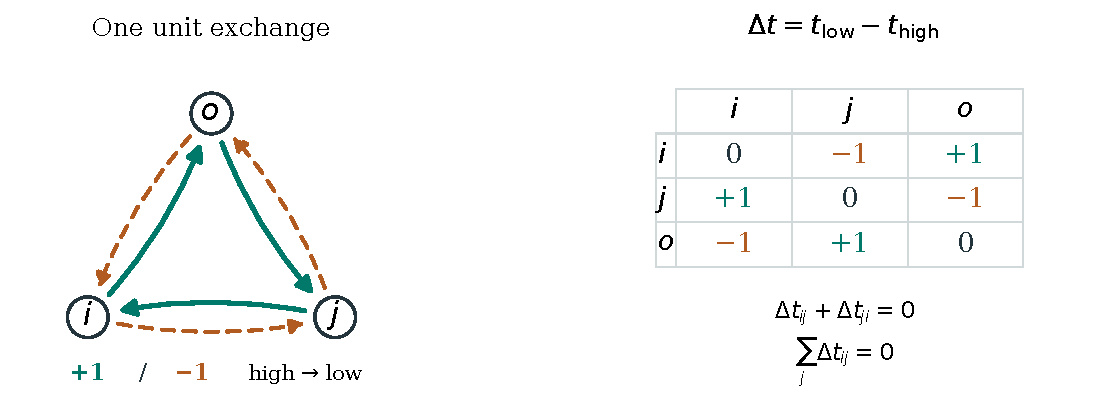
\includegraphics[width=\linewidth]{figures/circulation_en.pdf}
\caption{The change in type counts when a reserved copy switches from its high half to its low half. A directed entry counts blocks with the repeated color at its tail. Solid arrows add one block and dashed arrows remove one. The antisymmetric change has zero row sums, so all pair and row equations are preserved. This is a diagram of counts, not a drawing of the nine-point block system.}
\label{fig:circulation}
\end{figure}

Choose a sufficiently small constant \(\lambda>0\) depending only on \(k,\delta,\zeta\). For large \(n\), choose a prime \(p>8\) with \(\lambda n/4\le p\le\lambda n\). The placement has \(p^2\) copies per coordinate with pairwise disjoint sets of covered pairs. We call such a set a copy's pair footprint. The multi-color placement used here bounds the degree of their union by \(9p\); Paper I records a coarser bound for its placement. The vertex use fits inside the classes after requiring \(18(J+1)\lambda\le\delta\).

An explicit placement is as follows. Give each of the nine point positions its own pool indexed by the field with \(p\) elements. For \((u,v)\) in that field squared, place position \(\ell\) at pool coordinate \(u+\ell v\), for \(\ell=0,\ldots,8\). Two occupied pairs in the same pools determine \((u,v)\) uniquely, because their distinct slopes differ by a nonzero field element. Thus the footprints are disjoint. Each point belongs to \(p\) copies and has at most eight neighbors per copy, giving degree at most \(8p\le9p\). Use separate pools for the independent coordinates. Thus the vertex cost is linear in \(p\), while the supply of exchanges is quadratic.

Let \(L_Q\) be the pairs occupied by the prescribed packing, and let \(\Delta_Q\) be the maximum degree of the graph they form; Theorem 1.1 assumes \(\Delta_Q\le\gamma n\). Discard every exchange whose footprint meets \(L_Q\). Choose one pair of \(L_Q\) from each discarded copy. Because the footprints are disjoint, these witnesses are distinct. At most \(|L_Q|\) copies are discarded. If \(\gamma=\lambda^2/256\), then

\[|L_Q|\le n\Delta_Q\le\gamma n^2\le p^2/16.\]

Consequently the number \(s_i\) of usable copies on each coordinate satisfies \(p^2/2\le s_i\le p^2\). The retained exchange reserve avoids \(Q\).

\subsubsection{4.2. Center the residual target correctly}\label{center-the-residual-target-correctly}

Put every retained exchange in its high half, and let \(B_i\) be the resulting count on coordinate \(i\). Let \(\pi_i\) be the count in \(Q\). The desired seed mass on the graph outside both packings is

\[r_i=t_i-\pi_i-B_i+s_i/2.\tag{4.1}\]

To see the center in (4.1), suppose for a moment that the residual count were exactly \(r_i\). Attaching \(Q\) and every high half would give \(r_i+\pi_i+B_i=t_i+s_i/2\). We would reach the target by switching half the copies. The term \(s_i/2\) therefore centers the available integer corrections, while \(-\pi_i\) accounts for the blocks already prescribed in \(Q\).

The circulation basis extends the shift to the whole matrix while preserving all pair sums and row sums. Since \(B_i\le9p^2\) and \(\pi_i\le|Q|\le|L_Q|\), its coordinate size is at most \(10\lambda^2n^2\). The occupied-pair degree of \(Q\) and the baseline reserve together is at most

\[\Delta_Q+9p\le(\gamma+9\lambda)n\le18\lambda n.\]

Choose \(\lambda\) so that these two costs fit the seed-correction and interior-margin estimates of Section 3. The exact real-mass construction gives a diffuse seed of this actual residual graph with masses \(r_i\). The lattice, common-neighbor and hinge lemmas verify the other three conditions on that same graph.

\subsubsection{4.3. One approximate completion, then integer correction}\label{one-approximate-completion-then-integer-correction}

Apply T+ with tolerance \(\lambda^2/512\) and the \(J\) coordinate indicators. It yields one residual decomposition \(D_0\) with

\[|N_i(D_0)-r_i|\le\lambda^2n^2/512\le s_i/4\]

simultaneously for every coordinate. Attach \(Q\), obtaining a decomposition \(D_{\rm ext}\) outside the exchange footprints. Substitution of (4.1) gives

\[\left|N_i(D_{\rm ext})-(t_i-B_i+s_i/2)\right|\le s_i/4.\]

Subtract \(t_i-B_i\) in the last inequality. This places the integer \(z_i=N_i(D_{\rm ext})+B_i-t_i\) between \(s_i/4\) and \(3s_i/4\), hence between zero and the number \(s_i\) of available copies. Switch exactly \(z_i\) copies on coordinate \(i\) to their low half. Their footprints are unchanged, so the exchanges do not disturb \(D_{\rm ext}\) or one another. The final count on that coordinate is

\[N_i(D_{\rm ext})+B_i-z_i=t_i.\]

The pair and row identities now determine every other entry, by Section 2.2. This proves exact completion while retaining all blocks of \(Q\).

\begin{figure}[H]
\centering
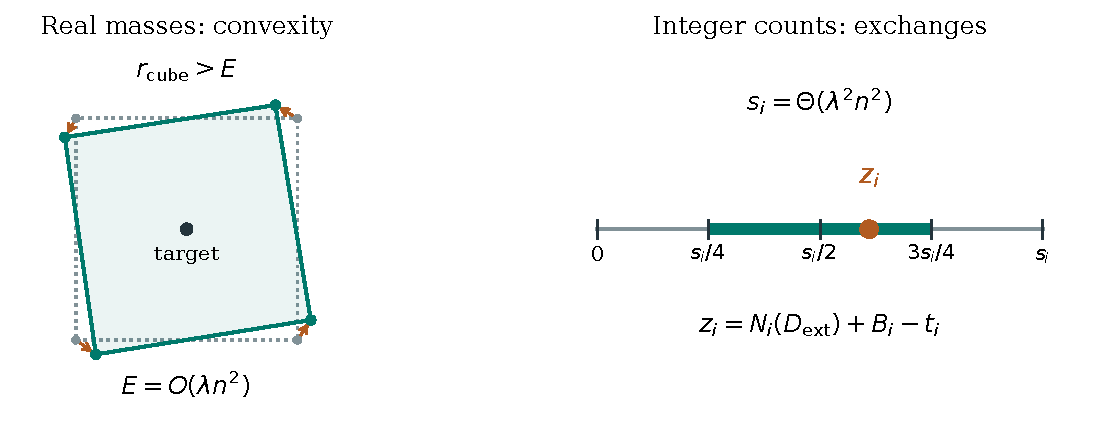
\includegraphics[width=\linewidth]{figures/two_scales_en.pdf}
\caption{The two corrections act on different scales. Left: in a schematic two-coordinate example, a cube of radius larger than the correction error still has the target inside the convex hull of its corrected corners. This gives exact real masses. Right: T+ leaves a smaller integer discrepancy, so the required number of switches lies between a quarter and three quarters of the available copies. The panels are not drawn to a common numerical scale.}
\label{fig:two-scales}
\end{figure}

The constants are chosen in the following order. We fix \(k,\delta,\zeta\), choose \(\lambda\) small enough for the seed and placement estimates, set \(\gamma=\lambda^2/256\), and choose the tolerance in T+. Only then do we take the maximum of the required order thresholds. The partition, matrix and packing are supplied afterwards. We do not assert a numerical value for \(n_0\).

We make no claim that this dependence is mild. As \(\delta\) decreases, the ratio \(R\) and the inverse constant \(K_c\) can grow; as the seed margin decreases, \(C_0\) grows. The displayed condition \(8K_cC_0^2\Delta\le n\) therefore forces a smaller deletion budget. The later choice \(\gamma\le\lambda^2/256\) makes the prescribed packing fit the exchange reserve as well. These are sufficient choices for fixed positive margins, not an optimized bound uniform down to zero margin.

\subsection{5. Counting inside each prescribed matrix}\label{counting-inside-each-prescribed-matrix}

The group-and-Latin-table construction below follows Wilson's counting scheme {[}11{]}. For unrestricted design counts, see Keevash {[}12{]}. Here the target matrix remains fixed throughout. The upper bound in Theorem 1.2 follows from Linial--Luria {[}6{]}: forgetting the colors and type counts injects our family into the family of all labeled Steiner triple systems. It remains to obtain the coefficient \(1/6\) in each fixed matrix, rather than in a matrix chosen afterwards by pigeonhole.

\subsubsection{5.1. A prescribed Latin outline still has many refinements}\label{a-prescribed-latin-outline-still-has-many-refinements}

Partition the rows, columns and symbols of a Latin square of order \(B\) into classes of sizes \(b_i\). An outline specifies the number \(M_{ijs}\) of entries in row class \(i\), column class \(j\) and symbol class \(s\). Its three families of marginals must equal \(b_ib_j\), \(b_ib_s\) and \(b_jb_s\). Hilton's outline construction {[}8{]} refines any such nonnegative integral outline to a Latin square. We impose zero outline entries on forbidden color triples.

Choose one refinement and remember only the symbol class in each cell. For a symbol class of size \(b_s\), the cells bearing that class form a \(b_s\)-regular bipartite graph on the \(B\) rows and \(B\) columns. Assigning its individual symbols is an ordered decomposition into \(b_s\) perfect matchings. Different symbol classes can be refined independently.

\Needspace{7\baselineskip}The permanent bound of Egorychev and Falikman {[}9,10{]}, applied after each matching is removed, gives at least

\[(d!)^B\left(\frac{B!}{B^B}\right)^d\]

ordered factorizations of a fixed \(d\)-regular bipartite graph. Indeed, when the remaining degree is \(d-r\), its adjacency matrix divided by \(d-r\) is doubly stochastic. Its permanent is at least \(B!/B^B\), so there are at least \((d-r)^B B!/B^B\) choices for the next matching. Multiplication over \(r=0,\ldots,d-1\) gives the displayed product.

The logarithm of that product is \(B\log(d!)+d\log(B!)-Bd\log B\). Applying \(\log(s!)\ge s\log s-s\) separately at \(s=d\) and \(s=B\) leaves \(Bd(\log d-2)\). For a symbol class, \(d=b_s\). Summing over classes uses \(\sum_s b_s=B\). Use \(\ell\) for a common lower bound on the symbol-class sizes, so it is distinct from the target matrix \(t\). If every \(b_s\ge\ell\), the resulting bound is

\[\log\#\{\text{refinements of this outline}\}
\ge B^2(\log\ell-2).\tag{5.1}\]

Refining symbol classes does not change the outline, since it keeps the class in every cell fixed. For this reason a prescribed type matrix does not reduce the leading entropy.

\subsubsection{5.2. Use one residual completion for all tables}\label{use-one-residual-completion-for-all-tables}

Let \(g\ge15\) be an admissible group order with \(2/g\le\zeta\), put \(\theta=2/g\), and choose a Steiner triple system on its \(g\) indices. A Wilson placement provides \(g\) groups of a common size \(B\), with common color multiplicities \(b_i\ge\ell\), and a reserve. The groups cover almost all vertices. On every block of the index system place a Latin table between its three groups.

All Latin tables cover the same cross-group pairs. Thus their common leftover graph can be completed once and the resulting completion retained for all later choices. If \(O=g(g-1)/6\) is the number of index blocks, choices of the \(O\) tables are independent. Each final system recovers its tables: the block containing a specified pair in the first two groups identifies its entry in the third. Hence the choices of tables map injectively to systems.

Exact types impose one further condition. Let \(\mathcal D_{\rm res}\) be the fixed completion, and write \(r_{ij}\) for its type counts. We will construct the Latin part from symmetric outlines, whose contribution to each directed type is a multiple of three. We therefore need

\[t_{ij}-r_{ij}\ge0,\qquad 3\mid(t_{ij}-r_{ij}).\tag{5.2}\]

Before completing, reserve boundedly many exchanges inside the vertex reserve. Their half choices repair the residues modulo three in the independent cycle coordinates. They leave the cross-group edge set fixed. The pair and row equations then give the residues for all other entries. The remaining graph is small enough that its number of blocks is at most \(\theta n^2\), while \(t_{ij}\ge\zeta n^2\); choosing \(\theta\le\zeta\) gives the first inequality of (5.2).

Set \(q_{ij}=(t_{ij}-r_{ij})/3\). Subtracting the identities of the completed system from (1.2) shows that

\[q_{ij}+q_{ji}=O b_ib_j,\qquad \sum_jq_{ij}=O b_i^2.\]

The integer splitting lemma divides \(q\) into \(O\) nonnegative matrices \(y^{(a)}\) satisfying the corresponding equations with \(O\) removed. The normalization by three reflects the three possible positions of the singleton color among the row, column and symbol classes of a Latin block. Each \(y^{(a)}\) produces a compatible outline whose type contribution is \(3y^{(a)}\). The tables can therefore vary independently, with total contribution \(3\sum_a y^{(a)}=t-r\).

Appendix A proves the splitting step. Appendix C constructs the balanced pattern, places it in the given partition, proves the residual seed and lattice conditions, and repairs the residues modulo three before any Latin tables are counted. Lemma C.2 proves the outline refinement with its support constraints. These constructions depend only on the hypotheses already stated.

\subsubsection{5.3. Recover the coefficient}\label{recover-the-coefficient}

With this choice of \(\theta\), the construction provides

\[gB\ge(1-\theta)n,\qquad \ell\ge n/C,\]

where \(C\) depends on \(g,k\) and the fixed margins, not on the partition or target. By (5.1) and the injection,

\[\log N(V_1,\ldots,V_k;t)\ge\frac{g(g-1)}6 B^2(\log\ell-2).\tag{5.3}\]

Divide by \(n^2\log n\). The bound \(\ell\ge n/C\) gives \((\log\ell-2)/\log n\ge1-(\log C+2)/\log n\). The bound on \(gB\) gives

\[\frac{g(g-1)B^2}{6n^2}\ge\frac16(1-1/g)(1-2/g)^2.\]

First choose a fixed admissible \(g\) large enough that the right-hand side is as close to \(1/6\) as required. Then increase \(n\) so that the logarithmic error is small. Together with the upper bound, this proves (1.4). The three-color case uses a three-class balanced pattern in the placement; it has the same residual and counting interface. No statement about all finite orders is needed.

\subsection{6. A profile at every large admissible order}\label{a-profile-at-every-large-admissible-order}

Theorems 1.1--1.3 apply to input data with margins. We now explain the separate construction of profiles needed for Theorem 1.4.

\subsubsection{6.1. Integer sizes near a real profile}\label{integer-sizes-near-a-real-profile}

Dividing the exact class-size identities by \(n\) and \(n^2\) suggests the real limiting constraints

\[p_i>0,\qquad \sum_i p_i=1,\qquad \sum_i p_i^2=1/3.\]

For the seed-feasibility argument we choose strict cut inequalities

\[\left(\sum_{i\in S}p_i\right)^2<3\sum_{i\in S}p_i^2
\quad(\varnothing\ne S\subsetneq\{1,\ldots,k\}).\tag{6.1}\]

For fixed \(k\) there are only finitely many nonempty proper subsets, so the strict inequalities have a positive common margin. This margin is used in the cut conditions of Gale's integral feasibility theorem {[}5{]}. After subtracting a small positive baseline from the desired directed allocations, Gale's theorem supplies the remaining allocations for sufficiently close integer profiles satisfying (1.1). Section 3 then verifies the complete-host hypotheses and applies T. Lemma D.1 gives the network, its capacities, and every cut inequality explicitly.

For \(k=d+2\ge5\), the profile used in the construction is

\[p=(A,A+r/2,r,r/2,\ldots,r/2^{d-1}).\]

Put \(s=\sum_{j<d}2^{-j}\), \(s_2=\sum_{j<d}4^{-j}\) and \(A=(1-rs-r/2)/2\). The sum of the coordinates is one. Their squared sum is \(1/3\) exactly when

\[F(r)=\frac{(1-rs)^2}{2}+\frac{r^2}{8}+r^2s_2-\frac13=0.\]

For \(d\ge3\), \(7/4\le s<2\) and \(21/16\le s_2<4/3\). Substitution gives \(F(9/100)\ge0\) and \(F(13/100)\le0\). Continuity gives a root in that interval. It also gives \(A>2r>0\).

To check the cuts, separate subsets containing zero, one or both large coordinates. For a subset of the geometric tail, its terms after the largest one sum to less than that largest term. Induction on the number of terms gives \((\sum 2^{-j})^2<3\sum4^{-j}\). If exactly one large coordinate is present, it is larger than the entire selected tail, since it exceeds \(2r\); expanding the square keeps the defect positive. If both are present, let \(D\) be the nonempty omitted tail. Subtract the selected square sum from the global identity to express the defect in (6.1) as

\[rP_D(2-rP_D)-3r^2Q_D,\]

where \(P_D=\sum_{j\in D}2^{-j}\) and \(Q_D=\sum_{j\in D}4^{-j}\le P_D\). Since \(P_D<2\) and \(5r<2\), this is positive. The finite cut verification supplies the required margin.

\subsubsection{6.2. Why rounding alone does not suffice}\label{why-rounding-alone-does-not-suffice}

Rounding all coordinates independently preserves their sum only approximately and destroys the exact quadratic equation (2.1). To repair both equations, first round the classes with indices at least four to even integers. Let their remaining sum and squared-sum targets be

\[w=n-\sum_{i\ge4}c_i,\qquad S_4=n(n+2)/3-\sum_{i\ge4}c_i^2.\]

We need four integers with sum \(w\) and squared sum \(S_4\). Put \(M=4S_4-w^2\). At admissible orders the chosen parities give \(M\equiv3\pmod8\). The arithmetic approximation theorem supplies

\[a^2+b^2+c^2=M\]

near the direction determined by the first four real coordinates. Then set

\[(c_0,c_1,c_2,c_3)=\frac14
(w+a+b+c,\ w+a-b-c,\ w-a+b-c,\ w-a-b+c).
\tag{6.2}\]

The representation has three odd coordinates. The profile has \(p_0+p_2=p_1+p_3\), so the target of the middle coordinate \(b\) is zero. Changing only the sign of \(b\), when necessary, makes \(w+a+b+c\) divisible by four without affecting the approximation. Lemma D.3 gives the rounding and sign argument. The other three numerators then have the same divisibility. Adding the four equations in (6.2) gives sum \(w\). Squaring and adding gives \(4\sum_{i<4}c_i^2=w^2+M=4S_4\). Their squared sum is \(1\) modulo four, so exactly one of the four integers is odd. The already rounded classes are even. Hence all cross products are even.

The approximation makes \(c_i/n\) as close to \(p_i\) as required; positivity and the strict cut margins survive. This completes the passage from the real profile to admissible integer data at every sufficiently large admissible order.

\Needspace{11\baselineskip}\subsubsection{6.3. The arithmetic theorem and the four-color case}\label{the-arithmetic-theorem-and-the-four-color-case}

The exact input proved by the arithmetic provider is: for every unit vector \(u\in\mathbb R^3\) and every \(\epsilon>0\), every sufficiently large integer \(M\equiv3\pmod8\) has an integer representation \(x_1^2+x_2^2+x_3^2=M\) with

\[|x_i-\sqrt M\,u_i|\le\epsilon\sqrt M\quad(i=1,2,3).\tag{6.3}\]

The squarefree input is Duke's spherical equidistribution theorem {[}17{]}; {[}7{]} places it in the broader theory of positive ternary forms. The formal provider {[}15{]} combines its squarefree version with quaternion rotations to handle square factors. Thus (6.3) records the assembled all-radii result, not a new classical equidistribution theorem. Lemma D.2 gives the precise inputs and the reduction. The odd-radius four-squares input is supplied by {[}16{]}; its proof uses the circle-method route described there, with Heath-Brown's framework {[}18{]}.

For four colors, use the prescribed radius \(M=n(n+8)/3\), which is integral and congruent to three modulo eight. Apply (6.3) at \(u=(1,0,0)\) with \(\epsilon=1/8\). It gives \(a\ge7\sqrt M/8\) and \(|b|,|c|\le\sqrt M/8\), hence

\[3(a^2+b^2+c^2)=n(n+8),\qquad 7|b|\le a,\quad7|c|\le a.\]

Appendix D.4 converts these inequalities to integer classes of size at least \(n/16\), with the exact pair identities. The explicit allocation there lies between \(1/400\) and \(1-1/400\) and satisfies every seed equation. Applying T gives the four-color case.

For \(k\ge5\), Sections 6.1--6.2 give the required input for T. Taking the maximum of the arithmetic and combinatorial thresholds proves Theorem 1.4. The arithmetic threshold is ineffective because the provider uses Siegel's theorem, and improving the explicit constants of the absorber does not remove that dependence.

\Needspace{18\baselineskip}\subsection{7. Different Pasch counts with the same exact matrix}\label{different-pasch-counts-with-the-same-exact-matrix}

\subsubsection{7.1. Complete one Latin packing}\label{complete-one-latin-packing}

Take the completion constant \(\gamma\) from Theorem 1.1 and set

\[a=\min\{1,\delta/4,\gamma/18\}.\]

For large \(n\), choose \(m=2^r\) with \(an/2<m\le an\) and \(r\ge2K+2\). Choose disjoint sets \(U,V\) of size \(m\) in one color class and \(W\) of size \(m\) in another. This is possible because \(2m\le\delta n\).

A Latin square \(L\) on these sets gives the packing

\[Q_L=\{\{u_i,v_j,w_{L(i,j)}\}:1\le i,j\le m\}.\]

It covers every pair between two of \(U,V,W\) once and no other pair. All its \(m^2\) blocks have the same type. Its occupied-pair degree is \(2m\). Since \(m\le an\) and \(a\le\gamma/18\), we have \(2m\le\gamma n\), as required by Theorem 1.1. Complete one such packing \(Q_0\) to an exact realization \(D_0\) and put \(\mathcal R=D_0\setminus Q_0\). For every other Latin square, \(D_L=\mathcal R\cup Q_L\) is a Steiner triple system with exactly the same matrix \(t\).

\subsubsection{7.2. Account for both mixed terms}\label{account-for-both-mixed-terms}

We classify a Pasch by how many of its blocks belong to \(Q_L\). The only possibilities are zero, one, two and four. Three is impossible: the three Latin blocks contribute three incidences in each reserved part, whereas every vertex of a Pasch has even total incidence. Its fourth block must therefore meet every part oddly, hence once. Such a block cannot belong to \(\mathcal R\), because its pairs between reserved parts were already covered by \(Q_0\).

Consequently

\[P(D_L)=P(\mathcal R)+I(L)+C_1(L,\mathcal R)+C_2(L,\mathcal R),\tag{7.1}\]

where \(I(L)\) counts intercalates: two rows and two columns whose four entries have the pattern \(x,y\) in one row and \(y,x\) in the other. Their four associated blocks form exactly the Pasch configurations contained in \(Q_L\). The term \(C_s\) counts configurations with exactly \(s\) Latin blocks. The two-block term can occur, so it is kept alongside the one-block term.

Fixing the table and varying its row and symbol permutations independently, any specified potential Latin block occurs with frequency \(1/m\). Two specified intersecting compatible blocks occur with joint frequency \(1/[m(m-1)]\). For a shared row or column, two distinct entries have two distinct symbol images. For a shared symbol, its preimage symbol determines one row in each of two columns, and those rows are distinct; the uniform row permutation has the same two-point frequency. This covers all three possible intersection parts.

The candidate bounds follow directly from pair uniqueness. For a configuration with one Latin block, call the other three blocks \(\mathcal R_1,\mathcal R_2,\mathcal R_3\). Their pairwise intersections are three distinct points \(x,y,z\). The blocks of \(\mathcal R\) covering \(xy,xz,yz\), if they exist, are unique; their third points recover the possible Latin block. Every configuration has an encoding by an ordered triple \((x,y,z)\), and each encoding recovers at most one configuration. Thus \(n^3\) bounds these candidates. We use the convenient weaker envelope \(27n^3\) below.

For a configuration with two Latin blocks, the two exterior blocks share a point \(x\), while the two Latin blocks share a different point \(u\). There are at most \(n\) blocks of \(\mathcal R\) through a fixed \(x\): their other points occur in disjoint pairs, since \(\mathcal R\) is a packing. Choose \(x\), an ordered pair of exterior blocks through it, and \(u\). This gives at most \(n^4\) choices. Their four remaining points must be split between the two Latin blocks. Each Latin block must meet both exterior blocks, giving at most two cross-matchings. Hence \(2n^4\), and therefore the coarser \(6n^4\), bounds these candidates. Requiring the proper reserved parts only reduces their number. Averaging over the two permutations now gives a relabeling with

\[0\le C_1+C_2\le E_{\rm mix}(n,m),\qquad
E_{\rm mix}(n,m)=\frac{27n^3}{m}+\frac{6n^4}{m(m-1)}.\tag{7.2}\]

Both mixed terms are averaged together, so one relabeling satisfies (7.2). No independence between their occurrences is asserted.

\subsubsection{7.3. Separate internal counts by more than the mixed error}\label{separate-internal-counts-by-more-than-the-mixed-error}

For \(0\le i<K\), take the addition table of

\[G_i=(\mathbb Z/4\mathbb Z)^i\times(\mathbb Z/2\mathbb Z)^{r-2i}.\]

All groups have order \(m\). An intercalate in an abelian addition table is determined by its initial row, initial column and a nonzero element \(h\) with \(2h=0\). Conversely the two repeated-symbol equations force that form. Each unoriented intercalate has four orientations, so

\[4I_i=m^2\bigl(|G_i[2]|-1\bigr)=m^2(2^{r-i}-1).\tag{7.3}\]

For \(i<j<K\), this gives \(I_i-I_j\ge m^3/(4\cdot2^K)\). Permuting rows and symbols preserves \(I_i\). Choose a good relabeling for each table by (7.2). Its completed system has Pasch count in

\[[P(\mathcal R)+I_i,\ P(\mathcal R)+I_i+E_{\rm mix}(n,m)].\]

To compare error and gap, use \(m\ge an/2\) in the first term of (7.2). In the second term, \(m\ge2\) gives \(m-1\ge m/2\), and hence \(m(m-1)\ge m^2/2\ge a^2n^2/8\). The two estimates give

\[E_{\rm mix}(n,m)\le54n^2/a+48n^2/a^2\le102n^2/a^2.\]

The gap is at least \(a^3n^3/(32\cdot2^K)\). For it to exceed the error it suffices that \(3264\cdot2^K<a^5n\); the construction uses the more convenient sufficient condition \(4096\cdot2^K<a^5n\). The intervals are then disjoint, proving Theorem 1.3. This comparison is between a cubic gap and a quadratic error, with \(a\) and \(K\) fixed before \(n\). The cases \(K=0,1\) need no separation argument.

\Needspace{24\baselineskip}\subsection{8. Questions beyond the interior regime}\label{questions-beyond-the-interior-regime}

The positive margin on every directed type is used in both the seed correction and the exact exchanges. Removing it leads to four different questions.

{\begin{longtable}[]{@{}
  >{\raggedright\arraybackslash}p{(\linewidth - 4\tabcolsep) * \real{0.3333}}
  >{\raggedright\arraybackslash}p{(\linewidth - 4\tabcolsep) * \real{0.3333}}
  >{\raggedright\arraybackslash}p{(\linewidth - 4\tabcolsep) * \real{0.3333}}@{}}
\toprule\noalign{}
\begin{minipage}[b]{\linewidth}\raggedright
Question
\end{minipage} & \begin{minipage}[b]{\linewidth}\raggedright
Result available here
\end{minipage} & \begin{minipage}[b]{\linewidth}\raggedright
What an extension must supply
\end{minipage} \\
\midrule\noalign{}
\endhead
\bottomrule\noalign{}
\endlastfoot
General boundary spectrum for \(k\ge4\) & Every compatible matrix with a fixed positive quadratic margin & A replacement for the interior seed and exchange routes when types vanish or become scarce \\
Three-color spectrum at every admissible order & The large-order interior result; Paper I gives the large-order spectrum {[}2{]} & A uniform construction covering the finite-order gap, rather than a succession of isolated witnesses \\
Counting and Pasch diversity on the boundary & Optimal leading count and distinct Pasch counts at the same exact interior matrix & Enough independent choices and local replacements while keeping all boundary quotas fixed \\
An effective universal order threshold & Existence for each fixed \(k\ge4\) & An effective substitute for the arithmetic step involving Siegel's theorem \\
\end{longtable}
}

The obstructions differ. A zero type can remove a route needed by an exchange even when an integral realization exists. Counting additionally requires that the completion preserve many choices. The last question is arithmetic: sharpening a combinatorial inverse alone does not make the present threshold effective.

A typed nibble could be useful for producing partial packings when positive types have smaller margins. To reach the boundary conclusions, one would still need a surviving integer certificate and enough supported exchanges to repair exact quotas. A lower-density packing estimate alone does not supply these two ingredients.

\subsection{Appendix A. Splitting the integer quotas}\label{appendix-a.-splitting-the-integer-quotas}

\Needspace{7\baselineskip}\textbf{Lemma A.1.} Let \(M\) be a nonnegative integer matrix on two finite index sets, with row sums \(h a_i\) and column sums \(h b_j\), where \(h\) is a nonnegative integer. Then \(M\) is the sum of \(h\) nonnegative integer matrices, each with row sums \(a_i\) and column sums \(b_j\). Every summand is zero wherever \(M\) is zero.

\emph{Proof.} Assume first that \(h>0\). The real matrix \(M/h\) has the required integral row and column sums. We round it to an integer matrix while preserving those sums and keeping each entry between its floor and ceiling, as follows. Form the bipartite graph of its nonintegral entries. Every nonisolated vertex has degree at least two: exactly one nonintegral entry at a row or column would contradict its integral sum. A finite graph with minimum nonzero degree at least two contains a cycle. On this even cycle, increase alternate entries and decrease the others by the largest positive amount that stays within the original floor and ceiling bounds. Each row and column on the cycle has one increase and one decrease, so its sum is unchanged. At least one entry becomes integral, and previously integral entries outside the cycle stay fixed. Repeat. The number of nonintegral entries strictly decreases, so the process terminates.

Call the resulting integer matrix \(X\). Its entries are nonnegative and at most \(M\): for an integer \(M_{ij}\ge0\), the ceiling of \(M_{ij}/h\) is at most \(M_{ij}\). Thus \(M-X\) is nonnegative, has row sums \((h-1)a_i\) and column sums \((h-1)b_j\), and we apply induction. When \(h=0\), every row sum is zero, hence every entry is zero, and the empty family is the required decomposition. A zero entry of \(M\) cannot receive a positive contribution in a sum of nonnegative matrices. This proves the support statement as well.

\Needspace{7\baselineskip}\textbf{Lemma A.2.} Suppose \(x_{ii}=0\), \(x_{ij}\ge0\) are integers satisfying

\[x_{ij}+x_{ji}=h b_ib_j,\qquad \sum_j x_{ij}=h b_i^2.\]

Then \(x\) is the sum of \(h\) nonnegative integer matrices \(y^{(a)}\) with zero diagonal, pair sums \(b_ib_j\) and row sums \(b_i^2\).

\emph{Proof.} Make an allocation matrix with rows indexed by unordered color pairs \(e=\{i,j\}\) and columns by colors. In row \(e\), put \(x_{ij}\) in column \(i\), \(x_{ji}\) in column \(j\), and zero elsewhere. Its row sum is \(h b_ib_j\). Its column sum at \(i\) is \(h b_i^2\). Apply Lemma A.1. Each summand is still supported only at the two ends of its row, because zeros are preserved. Read its entry at \((\{i,j\},i)\) as \(y^{(a)}_{ij}\). The row sums of the allocation matrix give the pair sums of \(y^{(a)}\); its column sums give the row sums of \(y^{(a)}\). Summing the entries over \(a\) recovers \(x\).

To apply this to Section 5.2, first divide the nonnegative residual quotas \(t-r\) by three. The congruence in (5.2) makes the quotient integral. Its pair sums and row sums have the form of Lemma A.2 with \(h=O\). This supplies all the matrices \(y^{(a)}\) used there, with no additional divisibility assumption on the individual summands.

\subsection{Appendix B. Correction on the residual graph}\label{appendix-b.-correction-on-the-residual-graph}

This appendix proves the two facts used in Section 3: small errors in edge loads can be corrected with bounded weights, and deleting a sparse allowed packing preserves the physical lattice condition. Real solvability and integer solvability are separate statements.

\subsubsection{B.1. A right inverse with its domain specified}\label{b.1.-a-right-inverse-with-its-domain-specified}

For an edge vector \(r\), put

\[\ell(r)=\sum_{e\text{ cross}}r_e-2\sum_{e\text{ internal}}r_e.\]

Every allowed triangle has one internal edge and two cross edges, so its incidence vector has \(\ell=0\). All norms below are maximum norms. Let \(A\) denote the edge--triangle incidence map.

\Needspace{7\baselineskip}\textbf{Lemma B.1.} Suppose every class has size at least \(c_\ast\ge4\) and \(n\le R c_\ast\), with \(R\ge1\). For three classes there is a linear map \(\Phi\) on \(\ker\ell\) such that \(A\Phi r=r\) and \(\|\Phi r\|\le400R^5\|r\|/n\). For \(k\ge3\) classes the same conclusion holds with constant \(K_c=|\operatorname{Trip}(o)|400R^6(1+4R^2)\) in place of \(400R^5\).

\emph{Proof for three classes.} Write their sizes as \(a,b,c\), and let \(D=\|r\|\). First cover the internal edges. For each class \(i\), choose a different class \(j\), and assign weight \(r_{uv}/c_j\) to each triangle \(uvw\) with \(u,v\in V_i\) and \(w\in V_j\). Its internal-edge load is exactly \(r_{uv}\). Each weight is at most \(D/c_\ast\) in absolute value. A cross edge receives contributions from at most its two endpoint classes, of total absolute value at most \(2RD\). The remaining vector is supported on cross edges, has \(\ell=0\), and has norm at most \(D'=(1+2R)D\).

For a cross matrix \(h\) between classes \(i,j\), separate its mean, its row and column deviations, and the remainder:

\[h_{uw}=C+f(u)+g(w)+h^0_{uw}.\]

Here \(C\) is the mean of all entries, \(f\) is the row mean minus \(C\), and \(g\) is the column mean minus \(C\). Thus \(f,g\) have sum zero and \(h^0\) has every row and column sum zero. Their absolute bounds are \(D',2D',2D',4D'\), respectively. The following weights realize the three nonconstant terms without adding any internal-edge load:

\[\begin{aligned}
 h^0:&\quad \psi_{uv,w}=\frac{h^0_{uw}+h^0_{vw}}{c_i-2},\quad u,v\in V_i,\ w\in V_j;\\
 f:&\quad \psi_{wz,u}=\frac{f(u)}{c_j-1},\quad w,z\in V_j,\ u\in V_i;\\
 g:&\quad \psi_{uv,w}=\frac{g(w)}{c_i-1},\quad u,v\in V_i,\ w\in V_j.
\end{aligned}
\tag{B.1}\]

For example, summing the first expression over \(v\ne u\) gives \(h^0_{uw}\), because the column sum of \(h^0\) is zero. Summing over \(w\) gives zero, because its row sums vanish. The other two checks use the zero sums of \(f\) and \(g\). Since \(c_\ast\ge4\), the total correction on a triangle has absolute value at most \(24D'/c_\ast\).

Only three constant cross loads remain, say \(C_{AB},C_{AC},C_{BC}\). Their compatibility is \(abC_{AB}+acC_{AC}+bcC_{BC}=0\). Use constant weights on each type, as follows:

\[\begin{gathered}
x_{AAB}=x_{AAC}=0,\qquad
x_{ABB}=\frac{C_{AB}}{b-1},\qquad x_{ACC}=\frac{C_{AC}}{c-1},\\
x_{BBC}=-\frac{a}{c}x_{ABB},\qquad
x_{BCC}=-\frac{a}{b}x_{ACC}.
\end{gathered}
\tag{B.2}\]

The internal loads vanish. The \(AB\) and \(AC\) loads are the desired constants, and the \(BC\) load is \(-aC_{AB}/c-aC_{AC}/b=C_{BC}\). These weights have norm at most \(2RD'/c_\ast\). Adding the three stages gives

\[\|\Phi r\|\le[1+(24+2R)(1+2R)]D/c_\ast\le79R^3D/n\le400R^5D/n.\]

All choices of successor classes are made once, so the construction is linear in \(r\).

This is an explicit construction of the inverse, with the sharper intermediate bound just obtained. The formal source uses finite averaging to prove the bound \(400R^5/n\) on the same compatible domain. The written proof is an alternative proof of the estimate used here, not a transcription of the formal construction.

\emph{Assembly for more classes.} Let \(\operatorname{Trip}(o)\) be all three-color subsets containing a chosen hub \(o\). Split each edge coordinate equally among the restrictions containing its endpoint colors. Call the resulting vectors \(G^0_\tau r\); their sum is \(r\) and each has norm at most \(\|r\|\). They need not individually satisfy the balance equation. Let \(z_0\) have total weight one, distributed uniformly on internal edges of the hub class. Since \(\ell(z_0)=-2\), set

\[G_\tau r=G^0_\tau r+\tfrac12\ell(G^0_\tau r)z_0.\]

Each \(G_\tau r\) has balance zero, and their sum is still \(r\), because \(\ell(r)=0\). The inequalities \(\|z_0\|\le4/c_\ast^2\) and \(|\ell(G^0_\tau r)|\le2n^2\|r\|\) give \(\|G_\tau r\|\le(1+4R^2)\|r\|\). The order of each restriction is at least \(c_\ast\), so replacing its order by \(n\) costs at most another factor \(R\). Apply the three-class inverse to each restriction and add. This gives precisely \(K_c\).

\Needspace{13\baselineskip}\subsubsection{B.2. Removing pairs without losing positivity}\label{b.2.-removing-pairs-without-losing-positivity}

\Needspace{7\baselineskip}\textbf{Lemma B.2.} Let an allowed packing occupy a pair set \(L\) of maximum degree \(\Delta\). Suppose the complete host has an exact seed \(\mu_0\) with \(1/(C_0n)\le\mu_0(T)\le C_0/n\), where \(C_0\ge1\). If \(8K_cC_0^2\Delta\le n\), its residual graph has an exact seed between \(1/(2C_0n)\) and \(2C_0/n\). For every test \(0\le w\le1\), its weighted mass differs from that of \(\mu_0\) by at most \((4K_c+1)C_0\Delta n\).

\emph{Proof.} Call a triangle bad when it contains an edge of \(L\), and good otherwise. Let \(b\) and \(g\) be restriction to bad and good triangles. Extend the residual edge indicator by zero on \(L\), and put \(d_0=1_{E\setminus L}-Ag\mu_0\). Then \(d_0\) vanishes on \(L\). It has balance zero, since \(L\) is a union of allowed triangles and every column of \(A\) has balance zero. A surviving edge belongs to at most \(2\Delta\) bad triangles: their third point is adjacent in \(L\) to one of its endpoints. Hence \(\|d_0\|\le2\Delta C_0/n\).

On the space of balanced vectors vanishing on \(L\), define \(R_0=Ab\Phi\). This operator preserves the space. Indeed, on an edge of \(L\) all incident triangles are bad, so \(Ab\Phi x=A\Phi x=x=0\). On a surviving edge there are at most \(2\Delta\) bad triangles, giving \(\|R_0x\|\le2\Delta K_c\|x\|/n\le\|x\|/2\). The convergent geometric series

\[x=\sum_{s\ge0}R_0^s d_0\]

satisfies \((I-R_0)x=d_0\) and \(\|x\|\le2\|d_0\|\). Set \(\psi=\Phi x\). Then \(Ag\psi=d_0\) and \(\|\psi\|\le4K_cC_0\Delta/n^2\le1/(2C_0n)\). Thus \(g(\mu_0+\psi)\) is the required positive seed. At most \(n^3\) triangle weights change, while at most \(n^2\Delta\) triangles are removed. Multiplying these numbers by the respective bounds on \(\psi\) and \(\mu_0\) gives \((4K_c+1)C_0\Delta n\). The same estimate works for every test between zero and one. This proves (3.2).

\Needspace{13\baselineskip}\subsubsection{B.3. An integer certificate using surviving triangles}\label{b.3.-an-integer-certificate-using-surviving-triangles}

\Needspace{7\baselineskip}\textbf{Lemma B.3.} Let the partition satisfy (1.1), and let \(H\) be the complete graph with the pairs of an allowed packing removed. Suppose that, in every color class, every set of at most \(k+4\) points has a common neighbor in \(H\) distinct from those points. Then \(1_{E(H)}\) is an integer combination of allowed triangles of \(H\).

For a deletion of maximum degree \(\Delta\), the neighbor assumption follows from \(c_i>(k+4)(\Delta+1)\). It also holds when every class contains more than \(k+4\) points adjacent to all other points.

\emph{Proof.} Work in the quotient of the free abelian group on \(E(H)\) by the subgroup generated by its allowed triangles. Write \(\chi(uv)\) for the image of a surviving edge. An allowed triangle gives the relation \(\chi(uv)+\chi(uw)+\chi(vw)=0\). We will prove that the sum of all edge images is zero.

First consider \(x,x',x''\) in one class, with all three internal edges present, and two points \(w,w'\) outside that class adjacent to all three. Subtracting the triangle relations gives \(D(x)+D(x')=D(x)+D(x'')=D(x')+D(x'')=0\), where \(D(x)=\chi(xw)-\chi(xw')\). Therefore \(D(x)=D(x')=D(x'')\) and \(2D(x)=0\). The same conclusion holds for any two points \(x,x'\) adjacent to \(w,w'\), even if \(xx'\) is missing. Choose a common neighbor \(y\) in their class and then auxiliary points completing the triples \(x,y,z\) and \(x',y,z'\), all adjacent to \(w,w'\). Each choice requires adjacency to at most four prescribed points. The preceding triangle calculation transfers the equality through \(y\).

Choose pairwise adjacent base points \(o_i\in V_i\), using the neighbor assumption successively. For \(v\in V_i\), choose \(w\) outside \(V_i\) adjacent to \(v,o_i\), and put \(\epsilon(v)=\chi(vw)-\chi(o_iw)\). The preceding difference calculation shows that this does not depend on \(w\). Applying it with the roles of the two classes reversed shows \(2\epsilon(v)=0\); also \(\epsilon(o_i)=0\). It follows that shifting an endpoint within its class changes an edge image by the difference of its two \(\epsilon\) values. When a base edge is missing we argue as follows. For a surviving \(uv\) with \(u\in V_i\), \(v\in V_j\), choose \(z\in V_i\) adjacent to \(u,o_i,v,o_j\) and distinct from them. To justify the first identity even when the edge \(o_iv\) is absent, choose an auxiliary point \(w\in V_j\), distinct from \(v,o_j\), adjacent to \(u,z,o_i\). The earlier difference calculation, applied to the outside points \(v,w\) and the inside points \(u,z\), gives \(\chi(uv)-\chi(zv)=\chi(uw)-\chi(zw)\). The definition of \(\epsilon\) using \(w\) makes the right-hand side \(\epsilon(u)-\epsilon(z)\). The other two identities use the present base edges. Thus

\[\chi(uv)-\chi(zv)=\epsilon(u)-\epsilon(z),\qquad
\chi(zv)-\chi(zo_j)=\epsilon(v),\qquad
\chi(zo_j)-\chi(o_io_j)=\epsilon(z).\]

Adding them gives the desired expression through the base edge, without using either \(o_iv\) or \(uo_j\). If an endpoint is already a base point, the corresponding identity is immediate. The choice of \(z\) imposes four adjacency requirements; the auxiliary choice of \(w\) imposes three. Excluding the named points uses at most \(k+4\) prescribed points in either choice, within the hypothesis of the lemma.

Put \(\beta_{ij}=\chi(o_io_j)\). For a surviving cross edge this gives \(\chi(uv)=\beta_{ij}+\epsilon(u)+\epsilon(v)\). For a surviving internal edge \(uv\subset V_i\), completing it with a point of another class gives \(\chi(uv)=-2\beta_{ij}+\epsilon(u)+\epsilon(v)\). The difference calculation at \(o_i\) shows that \(2\beta_{ij}\) is independent of \(j\); symmetry then makes it a single element \(\gamma\) for all class pairs. Set \(\kappa_{ii}=-\gamma\) and \(\kappa_{ij}=\beta_{ij}\) for \(i\ne j\).

Define a value on \emph{every} pair, including missing ones, by \(f(uv)=\kappa_{ij}+\epsilon(u)+\epsilon(v)\). On surviving pairs it equals \(\chi(uv)\). Over all pairs, the \(\epsilon\) contribution is \((n-1)\sum_v\epsilon(v)=0\), because \(n\) is odd. Since every \(c_ic_j\) is even, the class contribution is

\[\left(\tfrac12\sum_{i<j}c_ic_j-\sum_i\binom{c_i}{2}\right)\gamma=0,\]

where the last equality is (1.1). On any allowed triangle, whether or not its pairs survive, the sum of its three \(f\) values is \(-\gamma+2\kappa_{ij}+2(\epsilon(u)+\epsilon(v)+\epsilon(w))=0\). The deleted pairs are partitioned into such triangles. Subtracting their zero contribution from the sum over all pairs leaves \(\sum_{E(H)}\chi=0\), as required. This subtraction takes place in the residual quotient; it does not assume that a certificate in the original graph survives deletion.

\subsubsection{B.4. The two neighbor conditions}\label{b.4.-the-two-neighbor-conditions}

For H3, a prescribed third class contains at least \(c_i-2(\Delta+1)\) common neighbors of two roots. Here a root may exclude itself, and its missing neighbors exclude at most \(\Delta\) more points.

For H4, let \(uva\) and \(uvb\) be allowed triangles sharing exactly \(uv\). Choose \(p\) of the color of \(u\) and \(q\) of the color of \(v\), distinct from the four roots and from each other. Require all seven edges

\[uq,\ pv,\ pq,\ pa,\ pb,\ qa,\ qb\]

to be present. Their union \(J\) has two completions: \(J\cup\{ua,va\}\) decomposes as \(\{uqa,pva,pqb\}\), while \(J\cup\{ub,vb\}\) decomposes as \(\{uqb,pvb,pqa\}\). Every triangle has the type of one of the original triangles. Choosing \(p\) and then \(q\) leaves at least \((\delta n-4\Delta-5)^2\) choices. The edge set recovers \(p\) and \(q\) from the unique neighbors of \(v\) and \(u\) in \(J\), so these choices give distinct hinges. For small enough \(\Delta/n\) and large \(n\), there are at least \(\delta^2n^2/4\) hinges on exactly six vertices. This is the required power \(n^{6-4}\).

\subsection{Appendix C. The counting construction in full}\label{appendix-c.-the-counting-construction-in-full}

This appendix constructs the common residual completion used in Section 5. The Latin tables will vary only after that completion has been chosen.

\Needspace{13\baselineskip}\subsubsection{C.1. A balanced pattern fitting every large profile}\label{c.1.-a-balanced-pattern-fitting-every-large-profile}

\Needspace{7\baselineskip}\textbf{Lemma C.1.} For fixed interior and class margins and any sufficiently small fixed accuracy, all sufficiently large input profiles can be approximated by normalized positive integer vectors \(v\) satisfying \(3\sum v_i^2=(\sum v_i)^2\). A finite collection of such vectors suffices. For three colors one may use \(v=(1,1,1)\).

\emph{Proof.} A limit \(p\) of the normalized profiles has positive coordinates, sum one and \(3\sum p_i^2=1\). The allocations from Section 3 have subsequential limits \(a_{ij}\) bounded away from zero and one, with pair sums one and \(\sum_jp_ja_{ij}=p_i\). Consequently every nonempty proper subset satisfies

\[3\sum_{i\in S}p_i^2-p(S)^2=2\sum_{i\in S,j\notin S}p_ip_ja_{ij}>0.\]

For \(k\ge4\), let \(e\) be the indicator of any three colors, put \(Q(z)=3\sum z_i^2-(\sum z_i)^2\), and put \(\sigma(z)=\sum_{i\notin\operatorname{supp}(e)}z_i\). For a rational vector \(z\) close to \(p\), the rational vector

\[y=Q(z)e+6\sigma(z)z\]

satisfies \(Q(y)=0\). Indeed, \(Q(e)=0\) and the polar form at \((e,z)\) is \(-3\sigma(z)\), so the two remaining terms cancel. At \(z=p\), the vector is the positive multiple \(6\sigma(p)p\). Thus \(y/\sum y_i\) approximates \(p\), stays positive, and retains the strict cuts. Clearing denominators gives \(v\). The possible limits form a compact set with the fixed margins. Finitely many approximation neighborhoods cover it. All sufficiently large input profiles lie in their union; otherwise a convergent subsequence outside the union would have a limit inside it. This proves uniformity. For \(k=3\), the identity \(\sum_i(3c_i-n)^2=6n\) directly gives \(c_i/n\to1/3\).

The strict cuts also give an integer allocation with pair sums \(v_iv_j\) and row sums \(v_i^2\): send each pair's capacity \(v_iv_j\) to its two ends. The cut condition is \(\sum_{i\in S}v_i^2\ge\sum_{i<j\in S}v_iv_j\), which is precisely \(Q(v|_S)\ge0\). Total supply equals total demand. Gale's cut criterion {[}5{]} gives feasibility. With integer capacities, the augmenting-path argument of Ford--Fulkerson {[}21{]} gives an integer flow and hence the allocation. For three colors the cyclic allocation on \((1,1,1)\) does so explicitly.

Let \(g\ge15\) be fixed and admissible, and put \(\rho=1/(2g)\). Choose the accuracy \(\xi<\rho\delta/4\). For one of the finitely many patterns let \(M=\sum v_i\) and

\[\ell=\left\lfloor\frac{(1-\rho/2)n}{gM}\right\rfloor,\qquad b_i=\ell v_i,\qquad B=\ell M.\]

For large \(n\), place \(g\) disjoint groups with \(b_i\) points of color \(i\) in each. The approximation ensures \(c_i-gb_i\ge\rho\delta n/4\), so every color remains well represented in the reserve. Also \((1-\rho)n\le gB\le(1-\rho/2)n\) and \(\ell\ge n/(4g\max M)\). These inequalities justify the placement and the uniform constant in Section 5.3.

\Needspace{13\baselineskip}\subsubsection{C.2. Realizing an outline}\label{c.2.-realizing-an-outline}

\Needspace{7\baselineskip}\textbf{Lemma C.2.} Every nonnegative integral array \(M_{ijs}\) with the three pair marginals \(b_ib_j,b_ib_s,b_jb_s\) is the outline of a Latin square. If \(y_{ij}+y_{ji}=b_ib_j\) and \(\sum_jy_{ij}=b_i^2\), setting each of \(M_{iij},M_{iji},M_{jii}\) equal to \(y_{ij}\) and all other entries to zero gives an outline whose block counts are \(3y_{ij}\).

\emph{Proof.} This is Hilton's refinement {[}8{]}; the following splitting proof includes the required zero support. For each row class \(i\), apply Lemma A.1 to its matrix on column and symbol classes, splitting it into \(b_i\) matrices with row sums \(b_j\) and column sums \(b_s\). These are the individual rows. Now, for a column class \(j\), form the matrix on individual rows and symbol classes. Its row sums are \(b_j\) and its column sums are \(b_jb_s\). Split it into \(b_j\) matrices with row sums one and column sums \(b_s\). Each resulting cell now has exactly one symbol class, and each individual row and column has exactly \(b_s\) cells of that class. Those cells form a \(b_s\)-regular bipartite graph. Hall's condition follows by counting its edges from any set of rows, so it has a perfect matching. Remove one matching at a time and assign the distinct symbols. This produces a Latin square without changing any class counts or any zero entries. For the asserted symmetric outline, the diagonal marginals are \(\sum_jy_{ij}=b_i^2\), and the off-diagonal ones are \(y_{ij}+y_{ji}=b_ib_j\). Summing the three positions of the singleton gives \(3y_{ij}\).

\subsubsection{C.3. An exact seed on the common leftover graph}\label{c.3.-an-exact-seed-on-the-common-leftover-graph}

Let \(W_1,\ldots,W_g\) be the groups and \(W_\ast\) the vertex reserve. Delete all edges between distinct groups. The remaining graph \(H\) is the union of the complete graphs on \(W_a\cup W_\ast\). Write \(x=B/n\) and \(y=|W_\ast|/n=1-gx\); for large \(n\), \(0<y\le x\). The following weights distinguish only how many points of a triangle lie in the reserve:

\[w_2=w_3=\frac1{g(x+y)},\qquad w_1=\frac{1-yw_2}{x},\qquad w_0=\frac{1-yw_1}{x}.\tag{C.1}\]

They satisfy \(xw_0+yw_1=xw_1+yw_2=1\) and \(xw_2+yw_3=1/g\). Moreover \(w_1-w_2=(1-1/g)/x\ge0\) and \(w_0-w_2=(x-y)(w_1-w_2)/x\ge0\). Thus \(w_2\le w_j\le1/x\).

In the complete graph on \(W_a\cup W_\ast\), multiply the original type weight (3.1) by \(w_s\) when the triangle has \(s\) reserve points. The desired local edge load is one on edges meeting \(W_a\) and \(1/g\) on reserve edges. If the color proportions in both parts were exactly those of the full vertex set, (C.1) would give these loads, apart from the exclusion of the two roots. The discrepancy of a group color count from \(xc_i\) is at most \(xn\xi\), and that of the reserve count from \(yc_i\) is at most \(gxn\xi\). Since the original type weight is at most \(2/(\delta n)\), summing over colors and excluding roots bounds the local load error by

\[\epsilon\le\frac{2k(g+1)\xi}{\delta}+\frac{8k}{\delta nx}.\tag{C.2}\]

The target load is balanced exactly, not approximately. To check this, let \(b=(b_i)\), \(r=(c_i-gb_i)\) and \(d(z)=3\sum z_i^2-(\sum z_i)^2-2\sum z_i\). Expansion gives

\[g\,d(b+r)-(g-1)d(r)=d(gb+r)-g(g-1)Q(b)=0.\]

The last equality uses (1.1) and \(Q(b)=0\). It says precisely that the local target, with load \(1/g\) on reserve edges, has \(\ell=0\). The preliminary seed also has balanced incidence. Lemma B.1 therefore corrects its error. The local order is \((x+y)n\) and every local class has a fixed positive fraction of it. The preliminary weights are at least \((\eta/g)/((x+y)n)\) and at most \((4/\delta)/((x+y)n)\) for a fixed positive \(\eta\) coming from the interior margin. Choose \(\xi\) sufficiently small, then \(n\) sufficiently large, so that the inverse correction is at most half this lower bound. The corrected local seed is positive on all allowed triangles. Adding the \(g\) seeds gives load one on every edge of \(H\): a group edge occurs in one piece, and a reserve edge occurs in all \(g\) pieces with load \(1/g\) each.

For the lattice certificate, use the allocation of Lemma C.1 and the outline of Lemma C.2 to place one allowed Latin packing on every block of the index system. This covers exactly the deleted cross-group edges. The reserve provides the common neighbors required by Lemma B.3. It also supplies all free points in the hinge construction of Appendix B.4. Thus H2--H4 hold on \(H\), with constants depending only on the fixed parameters.

We will delete a bounded number of exchange footprints before applying T. The seed survives this deletion as follows. A bounded inverse on \(H\) is obtained by splitting edge vectors among its \(g\) complete pieces, giving each reserve edge share \(1/g\). Correct the balance of each share by the uniform vector on internal edges of one reserve color, exactly as in Lemma B.1. Each piece has linear class sizes, so the resulting inverse has norm at most \(K_H/n\) for a fixed \(K_H\). Lemma B.2 now applies with this inverse: its proof uses only the balance equation, a bounded inverse, and the bound \(2\Delta\) on bad extensions of a surviving edge. A bounded deletion has \(\Delta=O(1)\), so positivity holds for large \(n\). The remaining reserve also proves H2--H4. T therefore completes the graph after those exchanges have been set aside.

\subsubsection{C.4. Repairing residues before counting}\label{c.4.-repairing-residues-before-counting}

Reserve two vertex-disjoint copies of the nine-point exchange for each of the \(J\) independent coordinates, entirely inside \(W_\ast\). Complete the rest by C.3, attach every high half, and call the resulting type vector \(r^0\). For coordinate \(i\), switch the number \(z_i\in\{0,1,2\}\) congruent to \(r^0_i-t_i\) modulo three. Each switch decreases that coordinate by one and does not change the others. The resulting completion has \(r_i\equiv t_i\pmod3\) on the independent coordinates.

The omitted cross-group graph has \(6O b_ib_j\) edges between colors \(i,j\) and \(3O b_i^2\) edges inside color \(i\). Consequently \(t-r\) has pair sums \(3O b_ib_j\) and row sums \(3O b_i^2\). Reducing these equations modulo three, the cycle-coordinate argument of Section 2.2 gives divisibility for every entry. Also

\[|E(H)|\le gB^2/2+|W_\ast|n\le n^2/(2g)+\rho n^2=n^2/g.\]

Every residual block uses three of these edges, so \(r_{ij}\le n^2/(3g)\le(2/g)n^2\). Choosing \(2/g\le\zeta\) proves \(t-r\ge0\). Lemma A.2 then splits \((t-r)/3\), and Lemma C.2 realizes each summand. This completes all the constructions used in Section 5.

\Needspace{18\baselineskip}\subsection{Appendix D. The arithmetic passage to integer profiles}\label{appendix-d.-the-arithmetic-passage-to-integer-profiles}

\Needspace{13\baselineskip}\subsubsection{D.1. From strict cuts to a positive allocation}\label{d.1.-from-strict-cuts-to-a-positive-allocation}

\Needspace{7\baselineskip}\textbf{Lemma D.1.} Let \(p\) have positive coordinates, sum one, squared sum \(1/3\), and the strict cuts (6.1). Every sufficiently close normalized integer profile satisfying (1.1), at sufficiently large order, has an allocation \(a_{ij}\) bounded away from zero and one, with \(a_{ij}+a_{ji}=1\) and \(\sum_{j\ne i}c_ja_{ij}=c_i-1\).

\emph{Proof.} Choose \(\delta_0,\sigma>0\) so that every nearby profile has \(c_i\ge\delta_0n\) and every nonempty proper cut has \(3\sum_{i\in S}c_i^2-c(S)^2\ge\sigma n^2\). Choose a small fixed \(\eta_{\rm flow}>0\), and put \(B_0=\lceil\eta_{\rm flow} n^2\rceil\). We seek integer directed allocations \(x_{ij}\) with pair sums \(c_ic_j\), row sums \(c_i(c_i-1)\), and \(x_{ij}\ge B_0\). After paying \(B_0\) in each direction, pair \(ij\) has capacity \(e_{ij}=c_ic_j-2B_0\) and color \(i\) has demand \(d_i=c_i(c_i-1)-(k-1)B_0\).

Send each pair capacity to its two endpoint colors. Total capacity equals total demand by (1.1). Gale's feasibility criterion {[}5{]}, together with Ford--Fulkerson integrality {[}21{]}, requires that the demand on every subset be at least the capacity trapped inside it. The difference is

\[\sum_{i\in S}d_i-\sum_{i<j\in S}e_{ij}=\tfrac12\bigl(3\sum_{i\in S}c_i^2-c(S)^2-2c(S)\bigr)-|S|(k-|S|)B_0.\tag{D.1}\]

Choose \(\eta_{\rm flow}\le\min\{\delta_0^2/8,\sigma/(16k^2)\}\). For large \(n\), all capacities are nonnegative and (D.1) is positive for each proper nonempty subset. For the empty and full subsets it is zero. Thus an integral flow exists. Add back the baseline and put \(a_{ij}=x_{ij}/(c_ic_j)\). Because both directions have allocation at least \(B_0\), these ratios lie in \([\eta_{\rm flow},1-\eta_{\rm flow}]\). Dividing the row equation by \(c_i\) gives the required seed equation.

\subsubsection{D.2. All radii, including square factors}\label{d.2.-all-radii-including-square-factors}

We use two external analytic theorems in the following fixed-cap forms. First, Duke's theorem {[}17{]} gives: for every unit \(u\in\mathbb R^3\) and every positive accuracy, all sufficiently large squarefree \(d\equiv3\pmod8\) have an integer point of squared norm \(d\) approximating \(u\) to that accuracy after division by \(\sqrt d\). The precise formal interface is recorded in {[}15{]}. Second, the theorem {[}16{]} states that for every unit quaternion \(q\in\mathbb R^4\) and positive accuracy, every sufficiently large odd integer \(s\) has an integer quaternion \(\beta\) with \(\sum\beta_i^2=s\) and \(\beta/\sqrt s\) approximating \(q\) to that accuracy. Distribution of lattice points on spheres and ellipsoids has a classical literature, including Pommerenke {[}22{]}. The odd-radius statement used here is the one proved in {[}16{]}, by the circle method and Jacobi's formula; the historical reference does not replace it.

While their analytic proofs lie outside this article, the Lean endpoint remains unconditional because the selected source tree imports formal proofs of both inputs rather than leaving them as theorem hypotheses. In particular, its squarefree provider combines degreewise Weyl bounds with a representation lower bound using Siegel's theorem. The four-square provider combines a fixed-cap estimate with Jacobi's formula. The companion identifies these modules. These provider modules were compiled in the clean reconstruction described under Formal verification. Whether their formal statements faithfully express the cited analytic theorems still deserves specialist scrutiny; a compiled import and an axiom report do not replace that reading.

\Needspace{7\baselineskip}\textbf{Lemma D.2.} These inputs and Gauss--Legendre's three-squares theorem imply (6.3) for every sufficiently large \(M\equiv3\pmod8\).

\emph{Proof.} Write \(M=ds^2\) with \(d\) squarefree. Then \(s\) is odd and \(d\equiv3\pmod8\). For all \(d\) above the threshold in the first input, multiply the cap representation of \(d\) by \(s\).

There are only finitely many smaller \(d\). For each, Gauss--Legendre gives an integer vector \(v\) with squared norm \(d\). Let \(y=v/\sqrt d\). Choose a unit quaternion whose rotation sends \(y\) to \(u\). For \(y\ne-u\), normalizing the quaternion \((1+y\cdot u,y\times u)\) does this; for \(y=-u\), use a half-turn about an axis perpendicular to \(y\). Quaternion conjugation depends continuously on the quaternion, so the second input gives, for every sufficiently large odd \(s\), an integer \(\beta\) of squared norm \(s\) whose normalized rotation sends \(y\) as close to \(u\) as required. Regard \(v\) as a pure imaginary quaternion and put \(x=\beta v\overline\beta\). Its coordinates are integers, its real part is zero, and multiplicativity of the quaternion norm gives \(|x|^2=d s^2=M\). Its normalized direction is the desired one. Take the maximum rotation threshold \(S\) over the finitely many small \(d\). If \(D\) is the squarefree threshold, then \(M>D(S+1)^2\) ensures \(s>S\) whenever \(d<D\). This supplies one threshold for all \(M\), proving the lemma.

\subsubsection{D.3. The sign choice in the four remaining coordinates}\label{d.3.-the-sign-choice-in-the-four-remaining-coordinates}

For the profile of Section 6.1, put \(q=(p_0,p_1,p_2,p_3)\). It satisfies \(q_0+q_2=q_1+q_3\). The Hadamard coordinates of \(q\) are therefore

\[u_0=2(q_0-q_3),\qquad u_1=0,\qquad u_2=2(q_3-q_2).\]

Round the remaining coordinates to \(c_i=2\lfloor np_i/2\rfloor\). Each rounding error lies between \(-2\) and zero. With \(w,S_4,M\) as in Section 6.2, let \(\nu=u_0^2+u_2^2>0\). Expanding the sums gives \(w=n\sum_{i<4}q_i+O_k(1)\) and \(M=\nu n^2+O_k(n)\). Thus \(\sqrt M/n\to\sqrt \nu\). Apply Lemma D.2 in direction \((u_0,0,u_2)/\sqrt \nu\) with sufficiently small fixed accuracy. Then \((a,b,c)/n\) is as close to \((u_0,0,u_2)\) as required.

For admissible \(n\), the integer \(n(n+2)/3\) is \(1\) modulo four. The rounded tail has even entries, so \(S_4\equiv1\pmod4\) and \(w\) is odd. Therefore \(M=4S_4-w^2\equiv3\pmod8\), and \(a,b,c\) are all odd. If necessary, replace only \(b\) by \(-b\) to make \(w+a+b+c\) divisible by four. This changes that sum by two modulo four and preserves the approximation, because the target coordinate of \(b\) is zero. The other three numerators in (6.2) differ by twice a sum of two odd numbers, hence are divisible by four too. Formula (6.2) now supplies integers close to the required positive proportions. Its sum and squared-sum identities were checked in Section 6.2. Since their squared sum is \(1\) modulo four, exactly one of these four integers is odd. This proves all the parity conditions, and Lemma D.1 provides the seed.

\subsubsection{D.4. The four-color cap gives explicit margins}\label{d.4.-the-four-color-cap-gives-explicit-margins}

Let \(n\ge1000\) be admissible and take the representation in Section 6.3, with \(a\ge0\) and \(7|b|,7|c|\le a\). Define

\[f=(a+b+c,\ a-b-c,\ -a+b-c,\ -a-b+c).\]

The entries are odd and pairwise congruent modulo four. Choose \(s\in\{-1,1\}\) so that \(n+sf_0\) is divisible by four, and set \(c_i=(n+sf_i)/4\). They are integers and sum to \(n\). Also \(\sum f_i^2=4(a^2+b^2+c^2)\), giving \(3\sum c_i^2=n^2+2n\). The same congruence argument as in D.3 gives exactly one odd class.

From \(3a^2\le n(n+8)\) and \(n\ge1000\), squaring the positive bounds verifies \(12a\le7n\) and \(2400a\le1393n\). Hence

\[|f_i|\le9a/7\le3n/4,\qquad c_i\ge n/16,\qquad |c_i-c_j|\le4a/7\le199n/600.\]

Put \(a_{ij}=1/2+3(c_i-c_j)/(2n)\). Its values lie in \([1/400,1-1/400]\), and its pair sums are one. Finally,

\[\sum_{j\ne i}c_ja_{ij}=\frac{n-c_i}{2}+\frac{3}{2n}\left(c_in-\sum_jc_j^2\right)=c_i-1.\]

Thus (3.1) gives a diffuse exact seed with fixed margins, and Appendix B gives H2--H4 on the complete host. Applying T proves the four-color case without any additional profile assumption.

\subsection{Appendix E. The absorption theorems used here}\label{appendix-e.-the-absorption-theorems-used-here}

This appendix restates T and T+ from {[}4, §§1--2{]}. It fixes their complete input data; their proofs remain in {[}4{]}. The notation in this appendix is local. In particular, \(I\) is a label set and \(q\) is an exponent for the number of tests.

Let \(G\) be a finite simple graph on \(V\), with \(n=|V|\), a labeling \(\lambda:V\to I\), and a set \(\mathcal F\) of multisets of labels. No finiteness assumption on \(I\) is needed. Let \(\mathcal T\) be its allowed triangles: the three-element vertex sets whose three pairs are edges and whose label multiset belongs to \(\mathcal F\). A decomposition of an edge set is a family of allowed triangles with pairwise disjoint edge sets whose union is that edge set.

Let \(\alpha>0\), \(C\ge1\) and an integer \(h\ge6\) be given. The four conditions are as follows.

\textbf{H1 (exact diffuse seed).} There is \(\mu:\mathcal T\to\mathbb R\) such that

\[\frac1{Cn}\le\mu(Q)\le\frac Cn\quad(Q\in\mathcal T),\qquad
\sum_{Q\in\mathcal T:\ e\in E(Q)}\mu(Q)=1\quad(e\in E(G)).\]

Thus the lower bound applies to every allowed triangle, and the load equation to every actual edge.

\textbf{H2 (physical lattice).} In integer pair coordinates,

\[\mathbf1_{E(G)}\in\operatorname{span}_{\mathbb Z}
\{\mathbf1_{E(Q)}:Q\in\mathcal T\}.\]

The coefficients may be negative. Only triangles present in the graph may occur.

\textbf{H3 (typed common neighbors).} For every distinct \(u,v\in V\) and every label \(\ell\in I\) with \(\{\lambda(u),\lambda(v),\ell\}\in\mathcal F\) as a multiset,

\[|\{w\in V:uw,vw\in E(G),\ \lambda(w)=\ell\}|\ge\alpha n.\]

There is no assumption that \(uv\) is an edge.

\textbf{H4 (physical hinges).} Let \(T_a=\{u,v,a\}\) and \(T_b=\{u,v,b\}\) be any two allowed triangles sharing exactly the edge \(uv\). A hinge is an edge set \(J\subseteq E(G)\) disjoint from \(E(T_a)\cup E(T_b)\) such that both \(J\cup\{ua,va\}\) and \(J\cup\{ub,vb\}\) have allowed triangle decompositions. Its order is the number of vertices incident with \(J\). For every such root pair there is an integer \(i\), \(6\le i\le h\), for which at least \(\alpha n^{i-4}\) distinct hinges have order exactly \(i\). The four roots are fixed; hinges are counted as edge sets, not as enumerations of their vertices.

\Needspace{7\baselineskip}\textbf{Theorem T ({[}4{]}).} Fix \(I,\mathcal F,\alpha,C,h\) with \(\alpha>0\), \(C\geq1\) and \(h\geq6\). There is an integer \(n_0\) such that every labelled graph G of order \(n\geq n_0\) satisfying H1--H4 has an allowed triangle decomposition.

For the next statement, define the fractional target of a triangle function by

\[M_\mu(w)=\sum_{Q\in\mathcal T}\mu(Q)w(Q).\]

\Needspace{7\baselineskip}\textbf{Theorem T+ (triangle-statistics form, {[}4{]}).} Fix \(I,\mathcal F,\alpha,C,h\) as in Theorem T, together with \(\eta>0\) and an integer \(q\geq0\). There is an integer \(n_0\) such that the following holds for every labelled graph G of order \(n\geq n_0\) and every specified seed \(\mu\) satisfying H1, provided H2--H4 hold. For every finite family \((w_j)_{j\in\mathcal J}\) with

\[|\mathcal J|\leq n^q,\qquad |w_j(Q)|\leq1\quad(j\in\mathcal J,\ Q\in\mathcal T),\]

there is one allowed triangle decomposition \(\mathcal D\) such that

\[\left|\sum_{Q\in\mathcal D}w_j(Q)-M_\mu(w_j)\right|\leq\eta n^2
\quad(j\in\mathcal J).\]

The threshold precedes the graph, the specified seed and the entire test family. The same decomposition satisfies every inequality. In Section 4 we use the independent type indicators as tests; since their number depends only on \(k\), we may take \(q=1\) and enlarge the order threshold. The tolerance is chosen before applying the theorem. This is the conclusion of \texttt{main\_\allowbreak{}theorem\_\allowbreak{}T\_\allowbreak{}with\_\allowbreak{}triangle\_\allowbreak{}monitors}, the declaration imported in this paper. Theorem 1.3 uses the Latin replacement proof of Section 7.

\subsection{Formal verification}\label{formal-verification}

The accompanying source selection exposes our four main results through the aggregate module \texttt{CDRIII}. Starting with no initial project build objects, all 1,305 selected non-Mathlib dependency modules and the aggregate compiled in an isolated reconstruction. Only the pinned external Mathlib ecosystem cache was reused; Mathlib itself was not rebuilt from source.

The four endpoint axiom queries report only \texttt{propext}, \texttt{Classical.\allowbreak{}choice} and \texttt{Quot.\allowbreak{}sound}. Before-and-after source hashes match, and the completed audit binds the compiled objects to the selected sources and final configuration. No Lean proof or mathematical hypothesis was changed. The companion records the archive SHA-256, exact declarations, commands and verification evidence.

The companion documents the formalization rather than replacing the proofs in this article, with Appendices A--D supplying the technical arguments. Cited external theorems are invoked under their stated hypotheses without reproducing their proofs.

\subsection{Acknowledgments}\label{acknowledgments}

The author is deeply grateful to his wife María Paz and his children Lucas, Juan Cristóbal, Francisca, Raimundo and Benjamín for their love, patience and support.

\subsection{Use of artificial intelligence and computational tools}\label{use-of-artificial-intelligence-and-computational-tools}

Claude, by Anthropic, and ChatGPT/Codex, by OpenAI, were used to explore and check arguments and to prepare the manuscript.

Certo {[}13{]} was used to explore finite instances, check identities and assess candidate constructions. These computations informed the development of the arguments; finite checks were not treated as proofs of universal statements.

The author remains responsible for the arguments, citations, code and presentation. No AI system is listed as an author.


\Needspace{10\baselineskip}
\subsection{References}\label{references}

\begingroup\small\raggedright

\begin{enumerate}
\def\labelenumi{\arabic{enumi}.}
\tightlist
\item
  C. J. Colbourn, J. H. Dinitz and A. Rosa. Bicoloring Steiner triple systems. \emph{Electronic Journal of Combinatorics} 6 (1999), R25. \url{https://doi.org/10.37236/1457}.
\item
  J. P. Traverso Gianini. The exact block-type spectrum in the Colbourn--Dinitz--Rosa problem. Paper I, 2026. \url{https://doi.org/10.5281/zenodo.23987251}.
\item
  J. P. Traverso Gianini. A proof of the Colbourn--Dinitz--Rosa conjecture. Paper II, 2026. \url{https://doi.org/10.5281/zenodo.23987256}.
\item
  J. P. Traverso Gianini. Triangle decompositions III: Physical typed absorption and prescribed statistics. 2026. \url{https://doi.org/10.5281/zenodo.23867836}.
\item
  D. Gale. A theorem on flows in networks. \emph{Pacific Journal of Mathematics} 7 (1957), 1073--1082. \url{https://msp.org/pjm/1957/7-2/pjm-v7-n2-p04-s.pdf}.
\item
  N. Linial and Z. Luria. An upper bound on the number of Steiner triple systems. \emph{Random Structures \& Algorithms} 43 (2013), 399--406. \url{https://doi.org/10.1002/rsa.20487}; author preprint \url{https://arxiv.org/abs/1108.5042}.
\item
  W. Duke and R. Schulze-Pillot. Representation of integers by positive ternary quadratic forms and equidistribution of lattice points on ellipsoids. \emph{Inventiones Mathematicae} 99 (1990), 49--57. \url{https://www.math.ucla.edu/~wdduke/preprints/lattice2.pdf}.
\item
  A. J. W. Hilton. Outlines of Latin squares. In \emph{Combinatorial Design Theory}, North-Holland Mathematics Studies 149 (1987), 225--241. \url{https://www.sciencedirect.com/science/chapter/bookseries/pii/S0304020808728895}.
\item
  G. P. Egorychev. The solution of van der Waerden's problem for permanents. \emph{Advances in Mathematics} 42 (1981), 299--305. \url{https://doi.org/10.1016/0001-8708(81)90044-X}.
\item
  D. I. Falikman. Proof of the van der Waerden conjecture regarding the permanent of a doubly stochastic matrix. \emph{Mathematical Notes} 29 (1981), 475--479. \url{https://doi.org/10.1007/BF01139954}.
\item
  R. M. Wilson. Nonisomorphic Steiner triple systems. \emph{Mathematische Zeitschrift} 135 (1974), 303--313. \url{https://doi.org/10.1007/BF01215371}.
\item
  P. Keevash. Counting designs. \emph{Journal of the European Mathematical Society} 20 (2018), 903--927. \url{https://doi.org/10.4171/JEMS/779}.
\item
  J. P. Traverso Gianini. Certo. Software. \url{https://github.com/jtraverso/certo-math}.
\item
  P. Keevash. Coloured and directed designs. In \emph{Building Bridges II}, Bolyai Society Mathematical Studies 28 (2020), 279--315. \url{https://arxiv.org/abs/1807.05770}.
\item
  J. P. Traverso Gianini. Formalization of Duke--Schulze-Pillot bounds and squarefree three squares in fixed caps. Palomar, version 2. \url{https://palomar-registry.org/entry.html?id=PALOMAR-2026-11-07-000007&version=2}.
\item
  J. P. Traverso Gianini. Four squares in caps, and Jacobi's four-square theorem for odd integers. Formal theorem package. \url{https://github.com/jtraverso/four-squares-in-caps}; \url{https://palomar-registry.org/entry.html?id=PALOMAR-2026-11-08-000002&version=1}.
\item
  W. Duke. Hyperbolic distribution problems and half-integral weight Maass forms. \emph{Inventiones Mathematicae} 92 (1988), 73--90. \url{https://doi.org/10.1007/BF01393993}.
\item
  D. R. Heath-Brown. A new form of the circle method, and its application to quadratic forms. \emph{Journal für die reine und angewandte Mathematik} 481 (1996), 149--206. \url{https://doi.org/10.1515/crll.1996.481.149}.
\item
  M. J. Grannell, T. S. Griggs and C. A. Whitehead. The resolution of the anti-Pasch conjecture. \emph{Journal of Combinatorial Designs} 8 (2000), 300--309. \url{https://doi.org/10.1002/1520-6610(2000)8:4\%3C300::AID-JCD7\%3E3.0.CO;2-R}.
\item
  M. J. Grannell and A. D. S. Lovegrove. Maximizing the number of Pasch configurations in a Steiner triple system. \emph{Bulletin of the Institute of Combinatorics and its Applications} 69 (2013), 25--35. \url{https://grannell.net/Papers/maxpasch.pdf}.
\item
  L. R. Ford, Jr.~and D. R. Fulkerson. Maximal flow through a network. \emph{Canadian Journal of Mathematics} 8 (1956), 399--404. \url{https://doi.org/10.4153/CJM-1956-045-5}.
\item
  Ch. Pommerenke. Über die Gleichverteilung von Gitterpunkten auf m-dimensionalen Ellipsoiden. \emph{Acta Arithmetica} 5 (1959), 227--257. \url{https://doi.org/10.4064/aa-5-2-227-257}.
\end{enumerate}

\subsubsection{Supplementary material}\label{supplementary-material}

\textbf{{[}S1{]}} Formalization companion and Lean source archive, deposited with this preprint under DOI \textbf{10.5281/zenodo.24201563}. The official location of the package is \texttt{preprints/\allowbreak{}PAPER\_\allowbreak{}III} in \url{https://github.com/jtraverso/cdr-steiner-preprints}. The companion is provided in English and Spanish alongside the manuscripts.

\endgroup

\end{document}
